\chapter{VTOL Transition}
\label{ch:VTOL}

\section{Introduction}

As discussed in the introduction, a VTOL is a vehicle that can take off and land vertically.
Quadplanes are a fairly common implementation of a VTOL, in part because of their relative simplicity compared to other VTOL designs.
Quadplanes are a combination of two standardized hardware implementations: an airplane and a quadcopter.
They also do not need a rotor tilting mechanism, which simplifies design complexity significantly.

Most small airplanes have a naturally stable airframe, which means that the craft returns to flying a gentle, straight trajectory if the pilot lets go of the controls.
For this reason, airplanes can be flown by direct control surface inputs, without a stabilization flight controller, although this still requires great skill.
On the other hand, most rotorcraft, such as quadrotors are not naturally stable aircraft.
It is very difficult for rotorcraft to be controlled by a pilot using direct actuator inputs. 
When a pilot is manually flying a quadrotor via remote control, control stick inputs map to relative position and angle controls, so even manual flying includes some sort of control input.

While recreational flying is certainly fun, most unmanned work requires some sort of autopilot to accurately control the aircraft.
There exist many open source autopilots available for public use, such as Ardupilot, Px4, Rosflight, and Betaflight.
These autopilots include controllers for a variety of aircraft, such as airplanes, quadrotors, airships, flying wings, and many VTOL designs.
They allow a pilot to manually control the aircraft while maintaining stability, as well as automatic trajectory tracking, such as waypoint following, orbiting, and spline tracking control laws.
One may refer to \cite{uav_book} and \cite{vtol_book} for more information on the development of full autopilot stacks.

Although these autopilots include control for VTOL aircraft, these control laws are somewhat inefficient as they underutilize the physical capabilities of the system.
For example, the Px4 controller for VTOLs aircraft controls the aircraft as either a rotorcraft or an airplane.
When taking off, the aircraft ascends to a set altitude in multicopter (rotorcraft) mode and then slowly start the forward motor, or slowly tilt the forward rotors forward, until sufficient airspeed for foward flight has been reached. 
The reverse happens during landing, where the aircraft slowly slows down until multicopter control takes effect, and the aircraft can descend.
These methods are shown in Fig. \ref{fig:Px4}, and a video of transitioning may be found at \href{https://www.youtube.com/watch?v=f81n0aXdvKc}{https://www.youtube.com/watch?v=f81n0aXdvKc} \cite{transition_video}.

\begin{figure}[htbp]
    \centering
    \begin{subfigure}{0.48\textwidth}
        \centering
        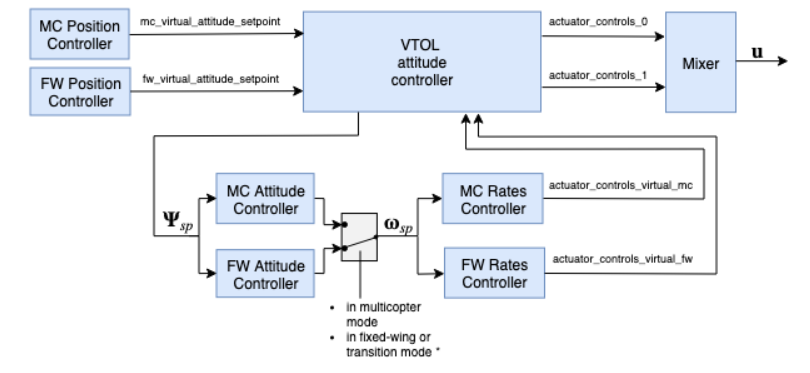
\includegraphics[width=\linewidth]{figs/chap1/Px4VTOL.png}
        \caption{Px4 VTOL control law. 
        Notice the switching mechanism from multicopter to forward attitude controls. 
      Modified from Px4 controller diagrams page \cite{px4_controller_diagrams}.}
        \label{fig:Px4ControlLaw}
    \end{subfigure}
    \hfill
    \begin{subfigure}{0.48\textwidth}
        \centering
        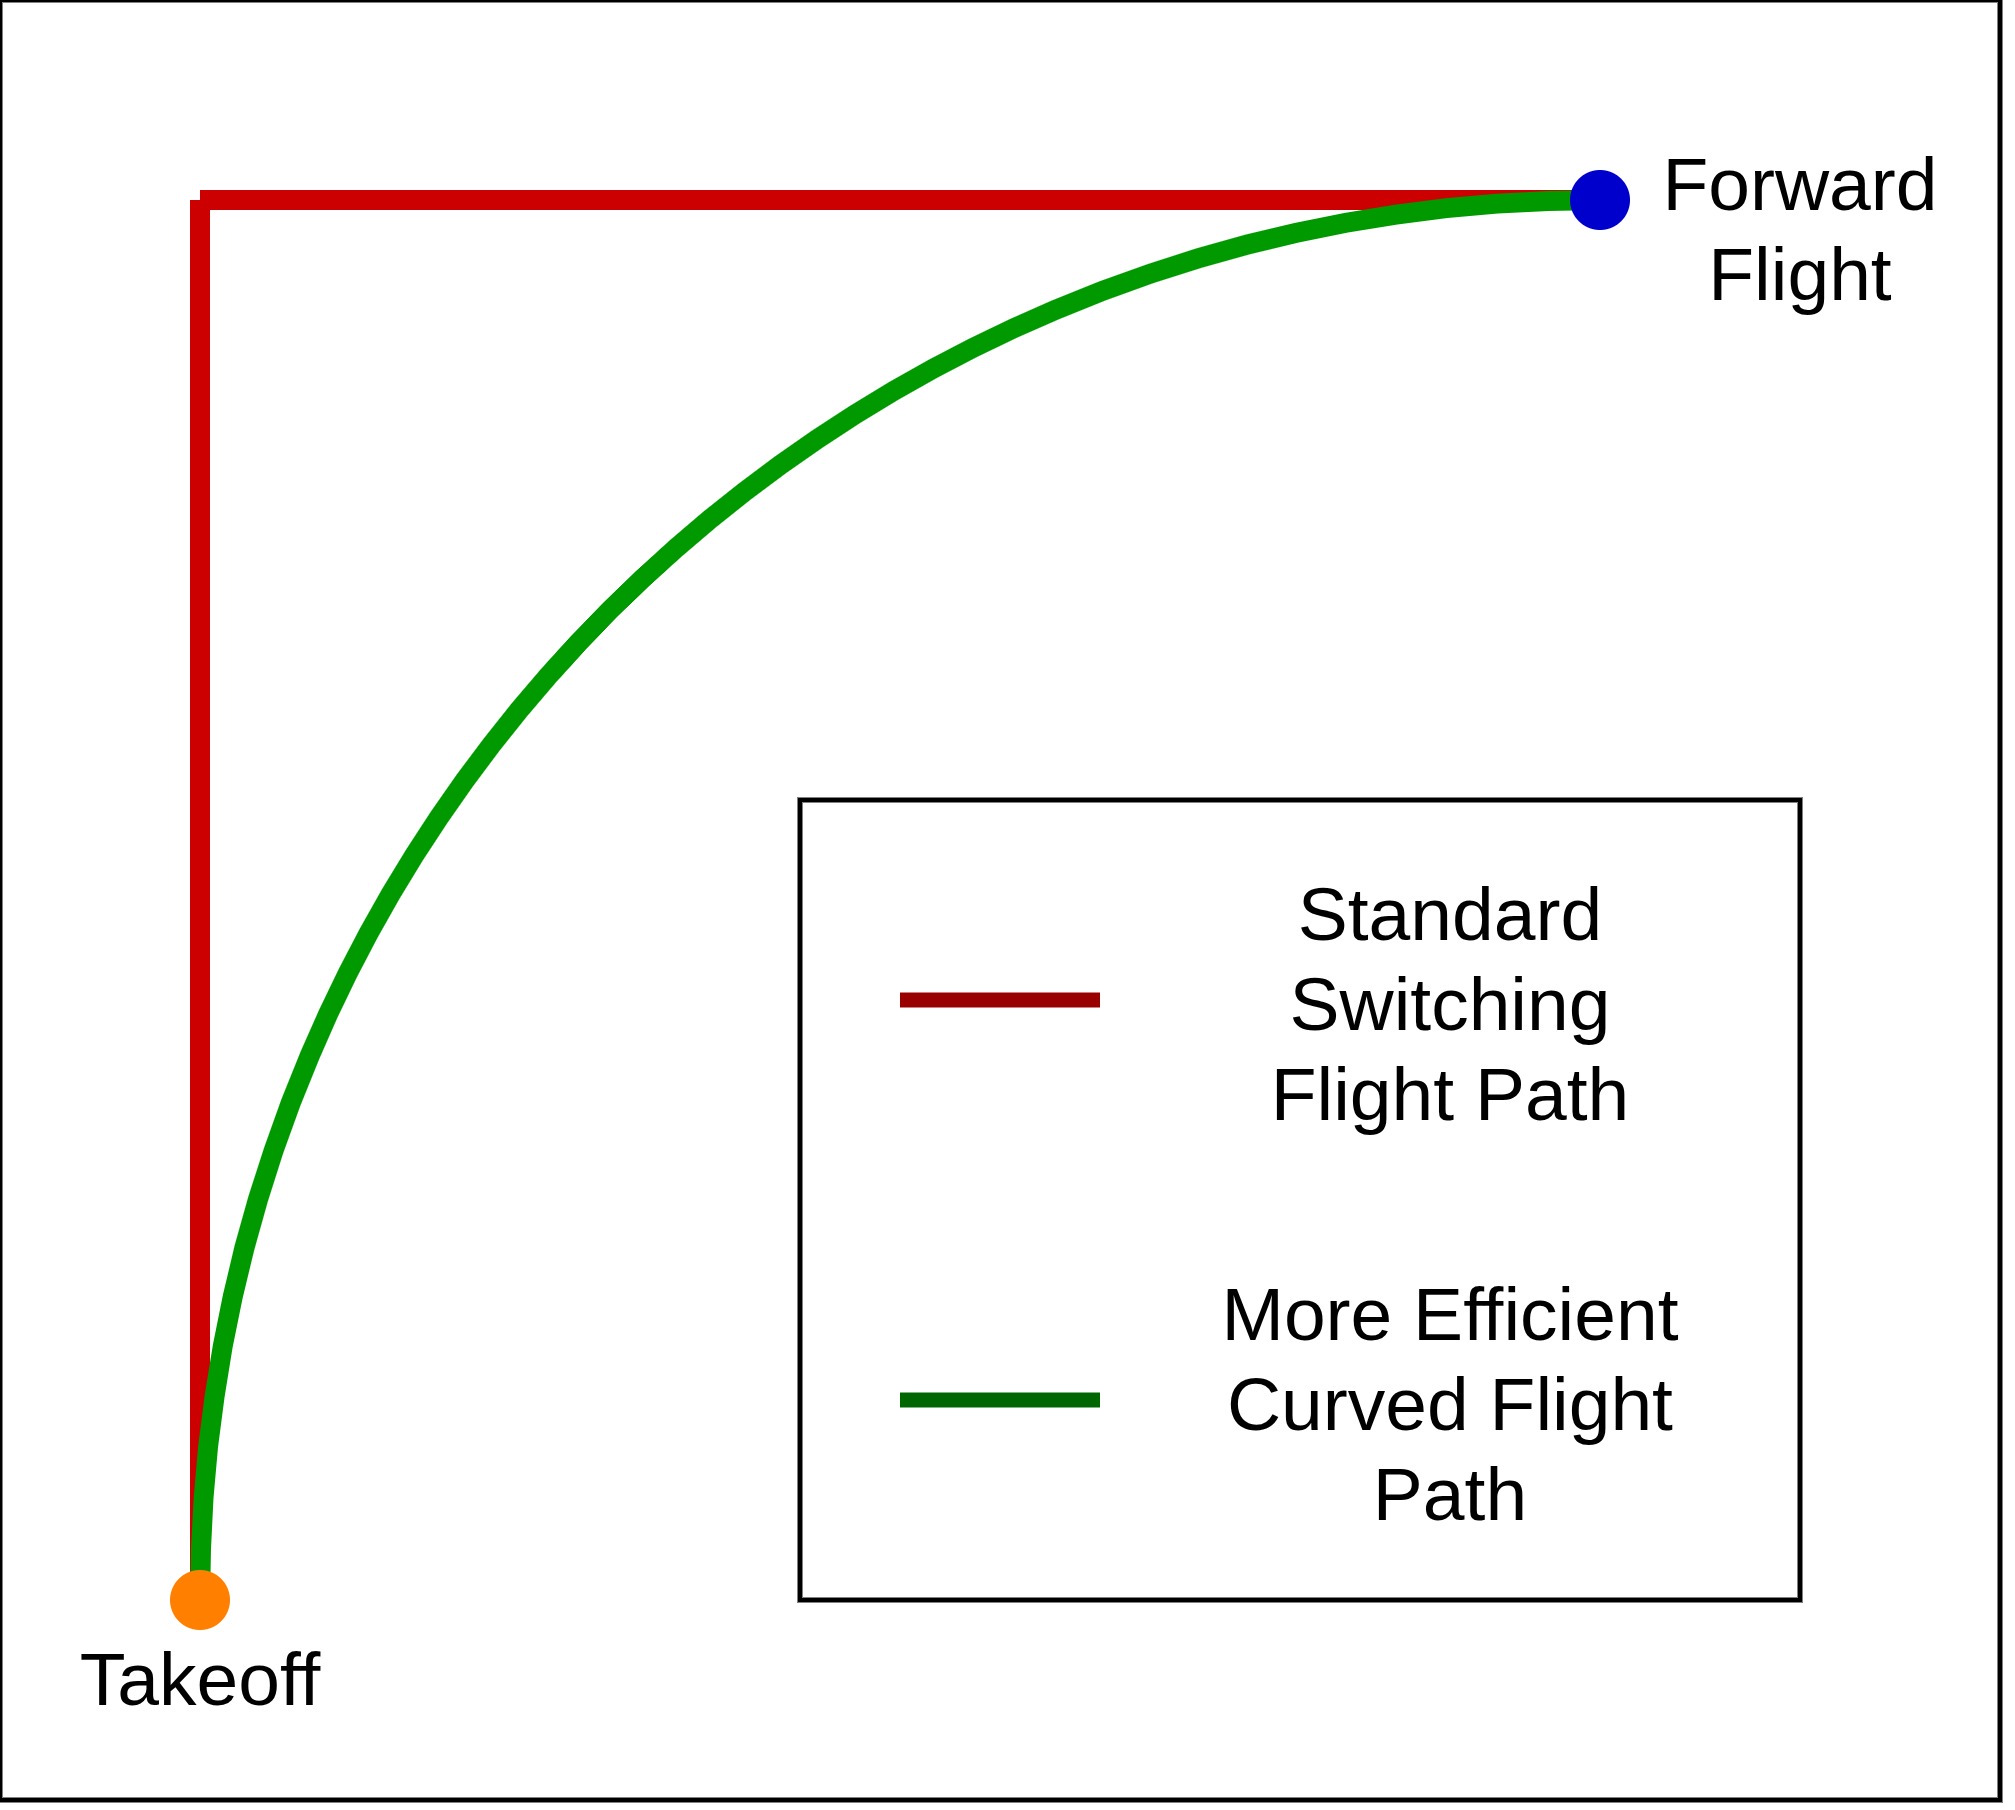
\includegraphics[width=\linewidth]{figs/chap1/Px4VTOLFlightPath.jpg}
        \caption{Flight path of Px4 controller compared with a more efficient path design.}
        \label{fig:Px4FlightPath}
    \end{subfigure} 
    \label{fig:Px4}
\end{figure}

While this method certainly works, it does not allow the aircraft to follow a generalized trajectory, nor does it utilize its actuators fully.
It is desirable to develop an autopilot that follows any general type of trajectory, such as a circle or a parabola.
The controller that is described in the following section generalizes the transition of the VTOL.
An autopilot for a VTOL quadplane is developed that is able to follow a spline trajectory while hovering as a multicopter, flying forward as an airplane, and transitioning in between the two.

\section{Literature Review}

Although the simplest and most common VTOL transition flight controller is described in the above section, hundreds of other flight control laws have been developed in control literature.
Several of these are reviewed in order to understand options for controlling VTOL controllers.

\subsection{Gain Scheduling}

One of the most prominent control methods for the transition of VTOL aircraft in particular, as well as all areas of aircraft experiencing nonlinearities is gain scheduling. 
Gain scheduling control of a nonlinear system is typically Jacobian linearization of a nonlinear system around numerous setpoints, typically equilibrium points, of the system \cite{gain_scheduling}.
In other words, it is linearization of the system around enough set states or operating regions of the sytem that the aircraft is expected to be able to stay controlled.
In the introduction, it was shown that the Px4 autopilot does a sort of binary gain scheduling between two operating points; more sophisticated gain schedulers simply use more operating points.


\subsubsection{Linear Parameter Varying Gain Scheduling}

A more advanced segmend of gain scheduling is linear parameter varying (LPV) gain scheduling, which means modification of the equations of motion and the controller gains using a varying parameter as the aircraft changes state.
The state transition equations become 

\begin{align}
    \dot{x} = A(\theta) x + B(\theta) u, \qquad y = C(\theta)x + D(\theta)u\\
\end{align}

where $\theta$ is a function of time or state of the aircraft.
As the VTOL changes its state during its transition, $\theta$ is altered accordingly, and the feedback matrix $K$ is updated using LQR, $H_\infty$, or another control law.
$\theta$ can be chosen to represent airspeed, angle of attach $\alpha$, tiltrotor angle, or some other similar control method.
For example, \cite{lpv_controller} presents an LPV controller for an octocopter plane using airspeed as the $\theta$ parameter.
Using this method, they are able to guarantee stability for the aircraft in the specified flight regime, though admittedly not through a full flight transition.

\subsection{Model Predictive Control}

Model Predictive Control (MPC) refers to a control method that iterates over short time intervals to bring the system to the desired state.
In other words, MPC finds a control input $u$ that brings the system state closer to a reference state by running an optimization algorithm for that time interval.
Because of this optimization, MPC converges on an optimal control input that takes into account all states and control inputs.
This method is particularly useful for nonlinear systems with highly coupled dynamics, such as a VTOL during transition.
A complete autopilot stack was developed in \cite{mpc_controller} for a tiltrotor VTOL, and was successfully implemented in hardware. 
Using the dynamic model of the aircraft, an optimization function was developed that finds optimal actuator controls $\bs{\delta}$ for controlling the VTOL as desired.
One section of the controller is an optimizer that finds the desired forces and moments that the should be actuated on the aircraft to take it to its desired trajectory.
Another optimizer then finds the actuator values and tiltrotor angles that controls the aircraft to obtain those desired forces and moments.

\subsection{Nonlinear Dynamic Inversion Controllers}

Nonlinear dynamic inversion, is essentially feedback linearization for control systems.
Feedback linearization cancels nonlinear dynamic terms in a system's dynamic equations of motion, which enables implementation of linear control laws for the system.
This means that the controller automatically actuates opposite to the undesired, nonlinear term to cancel it out and make the system better behaved. 
At each time step, the system is relinearized and an approximate state transition matrix is regenerated to be reinverted to drive the system to its desired state.
One of the first papers on aircraft NDI \cite{ndi_firstPaper} improved control of the F-18 in sumulation in very large angles of attack,  which tends to have very nonlinear effects.
They claim that using NDI allowed them to control the aircraft at angles of attack that would normally be outside the stability envelope for standard flight controllers.
NDI control requires that the system model is accurate so that a zeroing input actually removes undesired dynamic terms.
Incremental nonlinear dynamic inversion (INDI) attempts to solve this problem using incremental sensor data to actively estimate the aircraft dynamics. 
Doing so matches the controller to reality and reduces the probability of instability.

The large angles of attack during VTOL transition make INDI a particularly attractive solution as it can remove dynamic effects that would otherwise cause the craft to fail.
In \cite{incremental_nonlinear_dynamic_inversion}, two cascaded INDI flight controllers are used to control a quadplane in simulation, although it was not tested during transition.
An INDI controller is developed for VTOL hovering in \cite{nasa_hover}, and is continued for forward flight and transition in \cite{nasa_hover_2}.

\subsection{Motivation for 2D VTOL Model and Controller}

The solutions to the VTOL problem presented in the preceding section are all important parts of the attempt to control a VTOL aircraft during its transition phase.
In this paper, another solution to the VTOL transition problem is presented.
A 2D simplification of a VTOL simulation is developed to focus solely on transition control without stabilitation of degrees of freedom for roll, yaw, and east position.
This solution develops a differentially flat controller to make the quadplane track a B-Spline input trajectory.

\section{2D VTOL Dynamic Model}

This begins by simplifying a standard 3 dimensional dynamic design down to a 2 dimensional model. 
Early 3D attempts resulted in instability in the aircraft.
This begins with the following detail of the dynamics and mechanics of the aircraft operation in 2D.


\begin{figure}[htb]
    \centering
    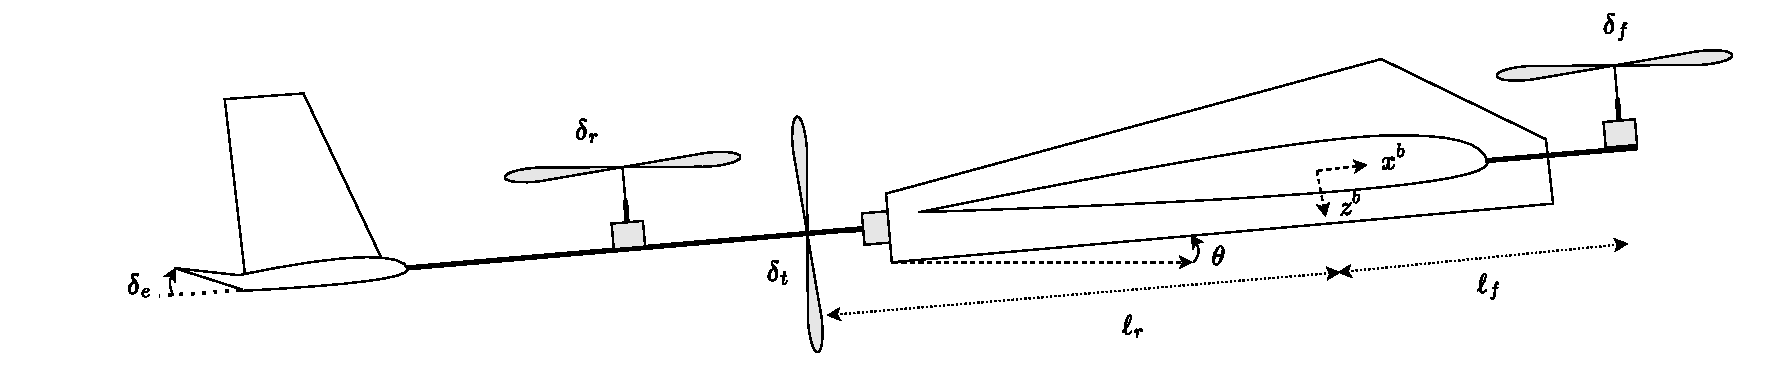
\includegraphics[width=0.75\linewidth]{figs/quadplane_2D.pdf}
    \caption{Geometry for 2D quadplane aircraft.}
    \label{fig:quadplane_2D}
\end{figure}

This model is represented by three degrees of freedom and their derivatives. 
These are north position ($p_n$), down position ($p_d$), and pitch ($\theta$) with their derivatives $\dot{p_n}$, $\dot{p_d}$, and $\dot{\theta}$ respectively. 
Velocity in the north and down directions are given as $v_n$ and $v_d$ respectively, while pitch rate is given $q$. 
These variables form the state vector as

\begin{align}
    x =
    \begin{bmatrix}
        p_n & p_d & \dot{p_n} & \dot{p_d} & \theta & \dot{\theta}
    \end{bmatrix}^\top\\
    =
    \begin{bmatrix}
        p_n & p_d & v_n & v_d & \theta & q
    \end{bmatrix}^\top
\end{align}.

\subsection{Actuators}

In this simplification, the planar VTOL has three rotors: two mounted vertically and one mounted horizontally. The vertically oriented rotor on the front of the craft is denoted in subscript by $f$, the vertically oriented rotor on the rear by subscript $r$, and the horizontally-oriented thruster propeller by $t$. The elevator is the sole control surface and is denoted in subscript as $e$. The possible control ranges for these actuators are given as

\begin{align*}
    \vec{\delta} =
    \deltaCommands
    \in
    \deltaCommandsExtrema
\end{align*}.

That is, the elevator can swing between the positive and negatives of $\Bar{\delta_e}$, while the throttles can assume values between zero and one. 
The rotor normal vectors, or thrust directions, are given in the body frame:

\begin{align}
    \hat{n}^b_{f} =
    \begin{bmatrix}
        0\\
        -1\\
    \end{bmatrix}
    \qquad
    \hat{n}^b_{r} =
    \begin{bmatrix}
        0\\
        -1\\
    \end{bmatrix}
    \qquad
    \hat{n}^b_{t} =
    \begin{bmatrix}
        0\\
        1\\
    \end{bmatrix}
\end{align}

\subsection{Equations of Motion}

Dynamic equations of motion relate the state of a system $x$ and that system's control inputs $u$ to the derivative of the state vector $\dot{x}$ for the general nonlinear case and the special linear case as

\begin{align}
  \dot{x} = f(x,u)\\
  \dot{x} = Ax + Bu
\end{align}

Let $\bs{p}_{a/b}^c\in\mathbb{R}^2$ and $\bs{v}_{a/b}^c\in\mathbb{R}^2$ represent the north and down position and velocity vectors for the state of the eVTOL. They are the position and velocity of frame $a$ relative to frame $b$ expressed in frame $c$. In this paper, $i$ represents the inertial or world frame, and $b$ represents the body frame of the aircraft. 

\begin{align}
    \bs{p}_{b/i}^i =
    \begin{bmatrix}
        p_n\\
        p_d\\
    \end{bmatrix}\\
    \dot{\bs{p}}_{b/i}^i =
    \begin{bmatrix}
        \dot{p}_n\\
        \dot{p}_d\\
    \end{bmatrix}\\
\end{align}

Let
\begin{align}
R_a^b(\vartheta)=
\begin{pmatrix}
    \cos\vartheta & \sin\vartheta \\ -\sin\vartheta & \cos\vartheta
\end{pmatrix}
\in SO(2)
\end{align}

denote the rotation from frame $a$ to frame $b$ by angle $\vartheta$. The rigid body equations of motion for the 2D quadplane are given by

\begin{subequations}
\label{eq:evtol_kinematics}
\begin{align}
\dot{\bs{p}}_{b/i}^{i} &= \bs{v}_{b/i}^{i} \\
\dot{\bs{v}}_{b/i}^i &= g \bs{e}_z^i + \frac{1}{m} R_b^i(\theta) \bs{F}^b \\
\dot{\theta} &= q \\
\dot{q} &= \frac{1}{J_y} M,
\end{align}
\end{subequations}

$\bs{F}^b \in \mathbb{R}^2$ is the non-gravitational force vector acting on the vehicle, expressed in the body frame. $R_b^i(\theta)$ is the rotation matrix to rotate a vector from the body frame to the inertial frame of reference. $M\in\mathbf{R}$ is the pitch moment or torque acting on the aircraft and $J_y$ is the rotational inertia of the aircraft about the $y$ or pitch axis. $\bs{e}_z^i=(0, 1)^\top$ is the direction of gravity expressed in the inertial or world frame, $g$ is acceleration due to gravity, which is $9.81 \frac{m}{s^2}$ and $m$ is the mass of the aircraft. The control vector in the body frame becomes: $\bs{u}^b=(\bs{F}^{b\top}, M)^\top$.

\section{A note on 3D to 2D Projections}
\label{sec:projections}

While developing this algorithm, there were many difficulties with the relationship between the equations of motion of a 3D aircraft and a 2D aircraft. Specifically, there needs to be a change of frames of reference between the two worlds. The aircraft operates within a 2D environment, which necessitates this change.

\subsection{3D Kinematics}

In the 3D frame, the position of an aircraft, with respect to a ground origin is given as its north, east, and down position, which is denoted as the vector in the inertial frame of reference:

\begin{align}
    p^i =
    \begin{bmatrix}
        n^i & e^i & d^i\\
    \end{bmatrix}
\end{align}

Given the Euler angles roll, pitch, and yaw ($\phi, \theta, \psi$), a rotation matrix is created which rotates this vector to describe the aircraft's body frame as $R_i^b$ or vice versa. 

A significant problem with the simulation environments is that they exist in 3D, with a 3D setup which is well defined. 
However, an environment with a 2D aircraft simulation existing in a 3D world is not well defined.
One approach is to create a system of dynamical equations where one component is constrained to be zero.

It is desirable to have a generalized 2D simulation existing in a 3D world in any particular coordinate frame, and not necessarily passing through the origin. 
That is, a 2D kinematic system may be defined on an arbitrary plane in the 3D world.

\subsection{2D Projections}
\label{sec:2DProjection}

A plane can be represented in 3D space with a known point on that plane and the vector normal to it.

An algorithm is set forth in \cite{duffBuildingOrthonormalBasis} on the creation of an orthonormal basis, where one member of that basis is already specified. That is, finding the basis for a plane when the vector normal to that plane is already specified. In this case, that specified member of the orthonormal basis is the vector normal or orthogonal to the plane.

The algorithm is given as


\begin{algorithm}
\caption{Orthonormal Basis Creation}
\begin{algorithmic}[1]
\State Input normal vector $\hat{n}$
\State Get components of $\hat{n}$: $n_x$, $n_y$, $n_z$
\State Get Sign of $n_z$. $$sign(n_z) = s_{n_z} = \{-1,1\}$$
\State Get helper variable $a$: $$a = \frac{-1}{s_{n_z} + n_z}$$
\State Get helper variable $b$: $$b = n_x n_y a$$
\State Get orthonormal basis vector $u_1$: 
$$u_1 = 
\begin{bmatrix}
    1 + s_{n_z} n_x^2 a\\
    s_{n_z} b\\
    -s_{n_z} n_x
\end{bmatrix}$$
\State Get orthonormal basis vector $u_2$:
$$u_2 =
\begin{bmatrix}
    b\\
    s_{n_z} + n_y^2 a\\
    -n_y
\end{bmatrix}
$$
\State Create full basis set $Q$:
$$
Q = 
\begin{bmatrix}
    \hat{n} & u_1 & u_2\\
\end{bmatrix}
$$
\State Create 2D basis $U$:
$$
U = 
\begin{bmatrix}
    u_1 & u_2\\
\end{bmatrix}
$$
\end{algorithmic}
\end{algorithm}.

This algorithm is particularly interesting because it creates a consistent orthonormal basis in 3D, including the $\hat{n}$ vector. But it also creates a 2D orthonormal basis out of $u_1$ and $u_2$. The basis $u_1$ and $u_2$ span a 2D plane in 3D space.

In order to have a plane that does not pass through the 3D origin, an offset vector is added to any point in 2D to the the corresponding 3D point. This offset vector $o_{3D}$ then becomes the origin on the 2D vector. The map between a 2D vector on the plane $v_{2D}$ and a 3D vector $v_{3D}$ is given as follows:

\begin{align}
    v_{3D} = U v_{2D} + O_{3D}
\end{align}

And then to map from a 3D point that sits on the plane to its 2D equivalent:

\begin{align}
    v_{2D} = U^+ (v_{3D} - O_{3D})\\
    U^+ = (U^\top U)^{-1} U^\top\\
\end{align}

Note that $U^+$ is the left pseudoinverse of $U$; it projects a 3D vector onto the plane to obtain its 2D equivalent. 
In general, a 3D vector does not lie on the plane, but must be projected onto the plane.
The component of the 3D vector that is orthogonal to the plane is removed, and then the projected vector is transformed from a 3D frame into a 2D frame. 
An example of plane projection is shown in Fig. \ref{fig:orthogonal projection}.

\begin{figure}
    \centering
    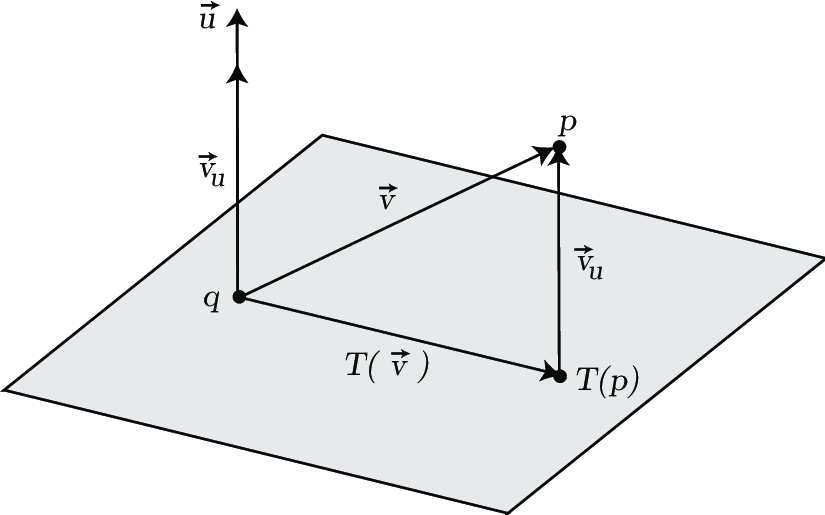
\includegraphics[width=0.5\linewidth]{figs/chap1/Orthogonal Projection.png}
    \caption{Projection of vector onto plane. \cite{orthogonal_projection_rg}}
    \label{fig:orthogonal projection}
\end{figure}

\subsection{2D VTOL application}

This mathematical tool represents the 2D quadplane in 3D space.
Apair of basis vectors must be found to represent the plane. 
The working plane needs to be defined in the North-Down plane, with zero component in the east direction. 
This limits the normal vector to be either $\hat{e}$ or $-\hat{e}$, that is, the positive or negative east vectors.
Two bases are obtained using the Pixar algorithm, which are

\begin{align}
    Q(\hat{e}) =
    \begin{bmatrix}
        0 & 1 & 0\\
        1 & 0 & 0\\
        0 & 0 & -1
    \end{bmatrix}\\
    Q(-\hat{e}) =
    \begin{bmatrix}
        0 & 1 & 0\\
        -1 & 0 & 0\\
        0 & 0 & 1
    \end{bmatrix}\\
\end{align}.

From these outputs, the latter is selected, because its north and down bases align with the north and down bases of the 3D case. 
It has the disadvantage of having its normal vector point in the negative $\hat{e}$ direction, but this doesn't affect anything.

To be clear, the actual equations of motion exist only in the 2D North-Down frame. 
A set of orthonormal basis vectors was created to facilitate that, and to be able to map back and forth between the two domains.



\subsection{Aerodynamic Forces and Moments}

Given the velocity vector $\bs{v}_{b/i}^b\doteq (u, w)^\top$, the airspeed $V_a$ and angle-of-attack $\alpha$ are computed as
\begin{align*}
  V_a(\boldsymbol{v}_{b/i}^b) &= \norm{\boldsymbol{v}_{b/i}^b} = \sqrt{\dot{p}_n^2+\dot{p}_d^2} \\
  \alpha(\boldsymbol{v}_{b/i}^b)  &= \angle{\boldsymbol{v}_{b/i}^b} =\tan^{-1}\left(\frac{\dot{p}_d}{\dot{p}_n}\right)\\
\end{align*}

Given the angle of attack $\alpha$, the rotation matrix from the wind to body frame is given by
\[
%    R_w^b(\boldsymbol{v}_{b/i}^b) = 
    R_w^b(\alpha) = 
    \begin{pmatrix}
        -\cos\alpha & \sin\alpha \\ 
        -\sin\alpha & -\cos\alpha
    \end{pmatrix}.
\]
Following ~\cite{uav_book}, it is assumed that the lift coefficient on the aircraft is given by
{\footnotesize\[
C_L(\alpha) = \left(1-\sigma(\alpha)\right) \left[C_{L_0} + C_{L_{\alpha}}\alpha \right] + \sigma(\alpha) \left[2\text{sign}(\alpha)\sin^2\alpha\cos\alpha \right],
\]}
where
\begin{equation} \label{eq:forces-sigmoid}
\sigma(\alpha) =  \frac{1+e^{-M(\alpha-\alpha_0)}+e^{M(\alpha+\alpha_0)}}{\left(1+e^{-M(\alpha-\alpha_0)}\right)\left(1+e^{M(\alpha+\alpha_0)}\right)} ,
\end{equation}
and $M$ and $\alpha_0$ are positive constants.
It is also assumed that the drag coefficient on the quadplane is given by
\[
C_D(\alpha) = C_{D_0} + C_{D_\alpha}\alpha + C_{D_{\alpha^2}}\alpha^2.
\]
Let
\begin{multline}
\bs{C} = (C_{L_0}, C_{L_{\alpha}}, M, \alpha_0, C_{L_q}, C_{L_{\delta_e}}, \\
    C_{D_0}, C_{D_\alpha}, C_{D_{\alpha^2}}, C_{D_q}, C_{D_{\delta_e}}, \\
    C_{M_{y0}}, C_{M_{y\alpha}}, C_{M_{yq}}, C_{M_{y\delta_e}}
    )^\top
\end{multline}
be the aerodynamic coefficients associated with the airframe. The aerodynamic forces are denoted as:

\begin{equation}
    \bs{F}^b(V_a, \alpha, q, \bs{C}) 
    = \bs{F}_0^b(V_a, \alpha, \bs{C}) 
    + \bs{F}_q^b(V_a, \alpha, \bs{C}) q 
\end{equation}

where

\begin{equation}
    \bs{F}_0^b(V_a, \alpha, \bs{C}) 
        = \frac{1}{2}\rho V_a^2 S 
            R_w^b(\alpha)
            \begin{pmatrix}
                -C_D(\alpha) \\
                -C_L(\alpha)
            \end{pmatrix}
    \label{eq:F_0}\\
\end{equation}

\begin{equation}
    \bs{F}_q^b(V_a, \alpha, \bs{C})
        =  \frac{1}{2}\rho V_a^2 S
            R_w^b(\alpha)\frac{c}{2V_a}
            \begin{pmatrix}
                -C_{D_q} \\
                -C_{L_q}
            \end{pmatrix},
    \label{eq:F_q}
\end{equation}

where $\rho$ is air density, $V_a$ is airspeed, $c$ is the mean wing chord. Similarly, from~\cite{uav_book}, the aerodynamic moment acting on the quadplane, with zero control inputs, is given by
\[
    M(V_a, \alpha, q, \bs{C}) 
        = M_0(V_a, \alpha, \bs{C}) 
        + M_q(V_a, \alpha, \bs{C}) q
\]
where
\begin{align*}
    M_0(V_a, \alpha, \bs{C}) 
        =  \frac{1}{2}\rho V_a^2 S 
            \left(
                cC_{M_{y0}} + cC_{M_{y\alpha}}\alpha
            \right) \\
    M_q(V_a, \bs{C})
        =  \frac{1}{2}\rho V_a^2 S \frac{c}{2V_a}
            \left(
                cC_{M_{yq}}
            \right).
\end{align*}


The following are the approximate total aerodynamic forces and moments experienced by the quadplane, with elevator control input. These are lift, drag, and pitching moment denoted $\bs{F}_{lift}$, $\bs{F}_{drag}$, and $M$. These equations are used later in the controller section to calculate desired forces and moments. 

\begin{align}
    \label{eq:totalAerodynamicForcesMoments}
    \bs{F}_{lift} = \frac{1}{2} \rho Va^2 S
    \begin{bmatrix}
        C_{L_0} + C_{L_\alpha} \alpha + C_{L_q} \frac{c}{2 V_a}q + C_{L_{\delta_e}} \delta_e
    \end{bmatrix}\\
    \bs{F}_{drag} = \frac{1}{2} \rho Va^2 S
    \begin{bmatrix}
        C_{D_0} + C_{D_\alpha} \alpha + C_{D_q} \frac{c}{2 V_a}q + C_{D_{\delta_e}} \delta_e
    \end{bmatrix}\\
    M_y = \frac{1}{2} \rho Va^2 S c
    \begin{bmatrix}
        C_{M_{y_0}} + C_{M_{y_\alpha}} \alpha + C_{M_{y_q}} \frac{c}{2 V_a}q + C_{M_{y, \delta_e}} \delta_e
    \end{bmatrix}
\end{align}

These equations are recombined as:

\begin{align}
    F^b_{a} = 
    \begin{bmatrix}
        -\cos(\alpha) & \sin(\alpha)\\
        -\sin(\alpha) & -\cos(\alpha)
    \end{bmatrix}
    \begin{bmatrix}
      \bs{F}_{drag}\\
      \bs{F}_{lift}
    \end{bmatrix}
\end{align}

\section{Differential Flatness}

Differential Flatness is the property that for a system defined by:

\begin{align*}
    \dot{x} = f(x,u)\\
    z = h(x)\\
\end{align*}

The state $x(t)$ and control inputs $u(t)$ can be reconstructed from the output $z$, and its derivatives: $\dot{z}$, $\ddot{z}$, etc as:

\begin{align*}
    x(t) = g_1 \left(z(t), \frac{d}{dt} z(t), ...\right)\\
    u(t) = g_2 \left(z(t), \frac{d}{dt} z(t), ...\right)
\end{align*}

In addition to this, the components of the output $z$ must not be differentially related over time. This means that the components of $z$ are not coupled together into a differential equation, for differential flatness to hold.

Of particular importance, $u(t)$ may be represented as a function of the system output $z(t)$.
For any given state of the system, with a reference input, a specific control input may be specified.
A trajectory that specifies the reference position, velocity, and acceleration for the craft can be directly related to a desired actuator output $\delta$ for each of the actuators. 
If that desired actuator output remains within the physical parameters of the actuators, then the actual system state can converge to the reference state. 

In order for this system to be differentially flat, the state variables $\bs{p}_{b/i}^i$, $\bs{v}_{b/i}^i$, $\theta$, $q$ and the input variables $\bs{F}^b$ and $M$ must all be expressed in terms of the flat outputs $\bs{z}_p^i$ and $z_\theta$ and their derivatives. 
That is, the current position $\bs{z}_p^i$ and pitch $z_\theta$ of the system are measured.

\begin{align}
    \bs{z} =
    \begin{bmatrix}
        \bs{z}^i_p\\
        z_{\theta}
    \end{bmatrix}
\end{align}

The position states are directly expressed in the flat outputs as $\bs{p}_{b/i}^i = \bs{z}_p^i(t)$.  The velocity states are directly expressed in the derivative of the flat outputs as $\bs{v}_{d/i}^i = \dot{\bs{z}}^i_p(t)$. The pitch angle and pitch rate are directly expressed in terms of the flat output as $\theta(t)=z_\theta(t)$, and $q(t)=\dot{z}_\theta(t)$.  The forces in the body frame are given by
\(
\bs{F}^b = R_b^{i\top}(z_\theta)\left(m\ddot{\bs{z}}_p^i - mg\bs{e}_z^i\right),
\)
and the moments are given by $M=J_y \ddot{z}_\theta$.
%
In summary, the equations are
\begin{subequations}
\label{eq:differential_flatness_equations}
\begin{align}
\bs{p}_{b/i}^i(\bs{z}) &= \bs{z}_p^i  \\
\bs{v}_{b/i}^i(\dot{\bs{z}}) &= \dot{\bs{z}}_p^i  \\
\theta(\bs{z}) &= z_\theta  \\
q(\dot{\bs{z}}) &= \dot{z}_\theta  \\
\bs{F}^b(\bs{z}, \dot{\bs{z}}, \ddot{\bs{z}}) &= R_b^{i\top}(z_\theta)\left(m\ddot{\bs{z}}_p^i - mg\bs{e}_z^i\right)  \\
M(\bs{z}, \dot{\bs{z}}, \ddot{\bs{z}}) &= J_y\ddot{z}_\theta. 
\end{align}
\end{subequations}.

All states and control inputs of the system may be found with a simple knowledge of the position $\bs{z}^i_p$ and pitch $z_{\theta}$. 
The real purpose of this exercise is to relate the reference output (where the aircraft shoule be) to a control input.
Take for example the moment control, $M = J_y \ddot(z)_{\theta}$.
If the input trajectory to the system provides a reference pitch $\theta$ for all timesteps, the moment that needs to be actuated on the aircraft may be calculated by taking the second derivative of theta.
This assumes that there is no error between the reference trajectory and the actual trajectory. 
The forces and moment vector equations are modified to take into account error between the reference output $z_{ref}$ and the actual output $z$.

\section{Pitch Free Trajectory Tracking}
\label{sec:PitchFree}

The first section of the controller is to determine the force the actuators need to exert on the aircraft. 
This is determined by the reference trajectory and the current state of the aircraft, at a particular point in time. 
The desired position from the reference trajectory, is given as $\bs{z}_{p,ref}^{i}$, with its derivatives for position and velocity as $\dot{\bs{z}}_{p,ref}^{i}$ and $\ddot{\bs{z}}_{p,ref}^i$ respectively. 
The advantage of using B-Splines for the reference trajectory is that they automatically produce this reference position, velocity, and acceleration. 
Each $\bs{z}_{ref}$ is a vector containing information position, velocity, or acceleration for north and down respectively.

\begin{align}
    \begin{bmatrix}
        \bs{z}_{p,ref}^{i}\\
        \dot{\bs{z}}_{p,ref}^{i}\\
        \ddot{\bs{z}}_{p,ref}^i\\
    \end{bmatrix}
    =
    \begin{bmatrix}
        \bs{p}(t)\\
        \frac{d}{dt}\bs{p}(t)\\
        \frac{d^2}{dt^2}\bs{p}(t)\\
    \end{bmatrix}
\end{align}

B-Splines and their temporal derivatives are discussed in section \ref{sec:BSplineMatrixRepresentation}.

Define the error variables
\begin{align*}
    \tilde{\bs{p}}^i &\doteq \bs{p}_{b/i}^i-\bs{z}_{p,ref}^i \\
    \tilde{\bs{v}}^i &\doteq \bs{v}_{b/i}^i-\dot{\bs{z}}_{p,ref}^i.
\end{align*}

These may be termed the differentially flat error variables. 
In other words, it is the difference between what the output state should be, and what the ouptut state actually is.

Differentiating and substituting equation \ref{eq:evtol_kinematics} gives:

\begin{subequations}
\label{eq:error_evolution_1}
\begin{align}
    \dot{\tilde{\bs{p}}}^i &= \bs{v}_{b/i}^{i}-\dot{\bs{z}}_{p,ref}^i \\
    \dot{\tilde{\bs{v}}}^i &= g \bs{e}_z^i + \frac{1}{m} R_b^i(\theta) \bs{F}^b-\ddot{\bs{z}}_{p,ref}^i.
\end{align}
\end{subequations}


Let $\bs{F}^i=R_b^i(\theta)\bs{F}^b$ be the force in the inertial frame, and selecting the feedback linearizing input as:

\begin{subequations}
\label{eq:inputs_feedback_linearization}
\begin{align}
    \tilde{\bs{u}}_F^i &= g \bs{e}_z^i + \frac{1}{m} \bs{F}^i-\ddot{\bs{z}}_{p,ref}^i,
\end{align}
\end{subequations}

gives
\begin{subequations}
\label{eq:error_evolution_3}
\begin{align}
    \dot{\tilde{\bs{p}}}^i &= \tilde{\bs{v}}^i \\
    \dot{\tilde{\bs{v}}}^i &= \tilde{\bs{u}}_F^i.
\end{align}
\end{subequations}

The net acceleration on the system is set to be the net control input $\tilde{\bs{u}}_F^i$. 
The system linear equations are then defined as

\begin{align}
    \tilde{\bs{x}}^i\doteq(\tilde{\bs{p}}^{i\top}, \tilde{\bs{v}}^{i\top})^\top
    \dot{\tilde{\bs{x}}}^i = A\tilde{\bs{x}}^i + B\tilde{\bs{u}}_F^i,
\end{align}

where

\begin{align*}
    A &= \begin{pmatrix} 
            0 & 0 & 1 & 0  \\
            0 & 0 & 0 & 1 \\
            0 & 0 & 0 & 0 \\
            0 & 0 & 0 & 0
         \end{pmatrix} \\
    B &= \begin{pmatrix} 
            0 & 0  \\
            0 & 0  \\
            1 & 0  \\
            0 & 1  
         \end{pmatrix}
\end{align*}.


Using LQR, design a linear control law as
\begin{equation}\label{eq:lqr}
    \tilde{\bs{u}}_F^i = -K \tilde{\bs{x}}^i
\end{equation}.

Rearranging Eq. \ref{eq:inputs_feedback_linearization} to solve for inertial force gives

\begin{align}
    \bs{F}^i = m \left[\ddot{\bs{z}}_{p}^i + \tilde{\bs{u}}_F^i - g \bs{e}_z^i\right]
\end{align}.

Combining Eqs. ~\eqref{eq:inputs_feedback_linearization} and~\eqref{eq:lqr}, and solving for the desired inertial frame forces gives
\begin{subequations}
\label{eq:input_final}
\begin{align}
    \bs{F}_{des}^i &= m\left[\ddot{\bs{z}}_p^i - g\bs{e}_z^i -K_F\tilde{\bs{x}}^i \right].
\end{align}
\end{subequations}.

This relates the desired acceleration on the aircraft $\ddot{\bs{z}}_p^i$, the gravitational acceleration vector $g\bs{e}_z^i$, and state (position and velocity) error $\tilde{\bs{x}}^i$ to the desired force control input $\bs{F}_{des}^i$. 
The net acceleration on the aircraft, which is generated by the actuators and the airfoil, needs to match the reference acceleration from the trajectory, overcome gravity, and bring the state error down to zero. 
The gain matrix $K$ is selected to tune the autopilot to its optimal performance. 


\section{Pitch Optimization Setup}

The next objective is to find the best pitch angle for a given desired force input given as $\bs{F}_{des}^i$. 
An appropriate body frame must be found to actuate the desired force that is given in the inertial frame. 
All of the body frame forces may be enumerated as

\begin{align}
    R_i^b(\theta)\bs{F}_{des}^i = \bs{F}_0^b + \bs{F}_q^b q + \bs{F}_{\delta_e}^b\delta_e + \bs{F}_p^b
\end{align}.

It is assumed that $\bs{F}_q^b q$ and $\bs{F}_{\delta_e}^b \delta_e$ are relatively small. 
To prove that this is the case, the autopilot was tested with the aircraft flying in standard fixed-wing mode at $V_a = 25 \frac{m}{s}$, and tracking a $20 \space m$ change every $25 \space s$, which produced the plot in Fig. \ref{fig:q_delta_e_omission}.

\begin{figure}
    \centering
    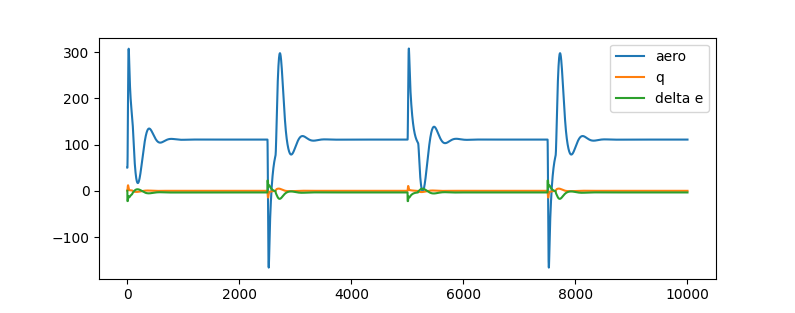
\includegraphics[width=0.75\linewidth]{figs/chap1/elevator and q force omission.png}
    \caption{Q and elevator lift force omission. The q and elevator terms in the force optimization portion are ommitted because their magnitudes are negligible compared to the lift from angle of attack.}
    \label{fig:q_delta_e_omission}
\end{figure}

For comparison, the average of the absolute value of the $\delta_e$ and $q$ terms are $4.0$ and $0.34$ newtons respectively, while the average for the $F_0$ term is $112$ newtons. 
While this is no proof, it shows a pattern of what is significant for the controller. 
Therefore, those terms are omitted from the above equation, which reduces down to

\begin{align}
    R_i^b(\theta)\bs{F}_{des}^i = \bs{F}_0^b(V_a, \alpha) + \bs{F}_p^b.
\end{align}.

Now, the angle of attack is given as: $\alpha = \theta - \gamma$, where $\gamma$ is the flight path angle. 
That is, it is the flight path angle of the craft as it is currently traveling, which is given as

\begin{align}
    \gamma = -\arctan\left(\frac{\dot{p_d}}{\dot{p_d}}\right)
\end{align}.

And where the desired flight path angle from the input trajectory is given as

\begin{align}
    \gamma_{des}(\dot{\bs{z}}_p) \doteq \tan^{-1}\left(\frac{-\dot{\bs{z}}_{d}}{\dot{\bs{z}}_{n}}\right)
\end{align}.


If all wind is zero, then

\begin{align}
    \alpha = \theta - \gamma
\end{align}

\section{Pitch Optimization}
\label{sec:PitchOptimization}

Solving for the desired propeller forces gives

\begin{align}
    \bs{F}_p^b = R_i^b(\theta)\bs{F}_{des}^i - \bs{F}_0^b(V_a, \alpha).
\end{align}

It is desirable to get as much of the net desired force as possible using the airframe and not the rotors.
Doing so minimizes energy expenditure and allows the aircraft to fly in fixed-wing mode as long as possible.
To achieve this, a desired pitch is now generated as 

\begin{equation}
    \label{eq:desired_propeller_force}
    \bs{F}_{p,des}^b(\theta, \dot{\bs{z}}_p, \bs{F}^i_{des}) = R_i^b(\theta)\bs{F}_{des}^i - \bs{F}_0^b\left(\norm{\dot{\bs{z}}_p}, \theta-\gamma_{des}(\dot{\bs{z}}_p)\right).
\end{equation}.

The desired forces to be acted on the aircraft in the inertial frame are already known, as are the current aerodyanmic forces acting on it, based on the state.
This equation finds the residual forces that must be actuated on the aircraft based on the current state and state error.
However, $\theta$ is not a fixed variable that is directly derived from the trajectory.
The pitch of the aircraft may be altered to maximize aerodynamic lift, and minimize needed rotor lift, given the current state of the aircraft.
The residual force equation is optimized with respect to $\theta$ to minimize the residual force needed from the rotors as

\begin{equation}
\label{eq:pitch_optimization}
\begin{aligned}
    &\text{Given}&& \dot{\bs{z}}_p, \bs{F}_{des}^i\\
    &\text{minimize} &&\|R_i^b(\theta)\bs{F}_{des}^i - \bs{F}_0^b\left(\norm{\dot{\bs{z}}_p}, \theta-\gamma_{des}(\dot{\bs{z}}_p)\right)\|_1 \\
    &\text{with respect to} && \theta\\
    &\text{subject to} 
    && \theta_{\min} \leq \theta \leq \theta_{\max} \\
     &&& |\theta - \theta_{\text{prev}} | \leq \Delta t q_{\max}
\end{aligned}.
\end{equation}

When this optimization function runs, it produces the reference pitch for the aircraft that optimizes its aerodynamic lift.
It also produces the reference for the residual forces to be compensated for by the vertical propellers.

\subsection{A Note on 1-Norm Minimization}
\label{sec:one norm}

The turning point for this controller is transitioning, which is changing from a multicopter controller into a fixed-wing controller. 
As discussed earlier, most of the other VTOL flight controllers in the literature actually use the two different flight controllers, and have a set of conditions which must be satisfied to change from one regime to the other.

The unique contribution of this chapter is a generalized flight controller that utilizes all of the lift-generating capabilities of the aircraft to follow a B-spline trajectory. 
As discussed above, at the beginning of the takeoff flight plane, the aircraft operates exactly like a 2D multicopter. 
It only uses the the two vertical rotors to generate lift and stabilize the aircraft. 
When the aircraft is flying at a constant airspeed in level flight, only the forward throttle and elevator are used, while the vertical rotors are all zero.

In between these two states, the aircraft uses all three of the rotors, as well as the elevator, to stay aloft. 
However, there is a very important point where the majority of the output switches from one regime to the other, which is called transition. 
Recall equation \ref{eq:pitch_optimization}, where given a current velocity $\dot{\bs{z}}_p$ and desired inertial frame force $\bs{F}_{des}^i$, it runs

\begin{align}
    &\text{minimize} &&\|R_i^b(\theta)\bs{F}_{des}^i - \bs{F}_0^b\left(\norm{\dot{\bs{z}}_p}, \theta-\gamma_{des}(\dot{\bs{z}}_p)\right)\|_1 \\
    &\text{with respect to} && \theta
\end{align}.

This minimizes the force required to be output from the quadrotors. 
The difference between the two forces is defined as

\begin{align}
    \bs{F}^b_{diff} = 
    R_i^b(\theta)\bs{F}_{des}^i - \bs{F}_0^b\left(\norm{\dot{\bs{z}}_p}, \theta-\gamma_{des}(\dot{\bs{z}}_p)\right)\
    =
    \begin{bmatrix}
        F^b_{n,diff}(\theta)\\
        F^b_{d,diff}(\theta)
    \end{bmatrix}
\end{align}.

The $1$ norm of a vector is the sum of the absolute value of the components of the vector, which is given as

\begin{align}
    v = 
    \begin{bmatrix}
        v_x\\
        v_y\\
        v_z\\
    \end{bmatrix}\\
    \|v\|_1 = \|v_x\| + \|v_y\| + \|v_z\|
\end{align}.

The optimization function then becomes

\begin{align}
        &\text{minimize} \quad  \|F^b_{n,diff}\| + \|F^b_{d,diff}\|
\end{align}.

An example of the 1-Norm is shown in Fig. \ref{fig:one norm visual}, comparing the 1-Norm and 2-Norm of a set of vectors. 
For any two vectors with the same 2-Norm magnitude, the vector which is more closely aligned to one of the axes has the smaller 1-Norm magnitude.

\begin{figure}
    \centering
    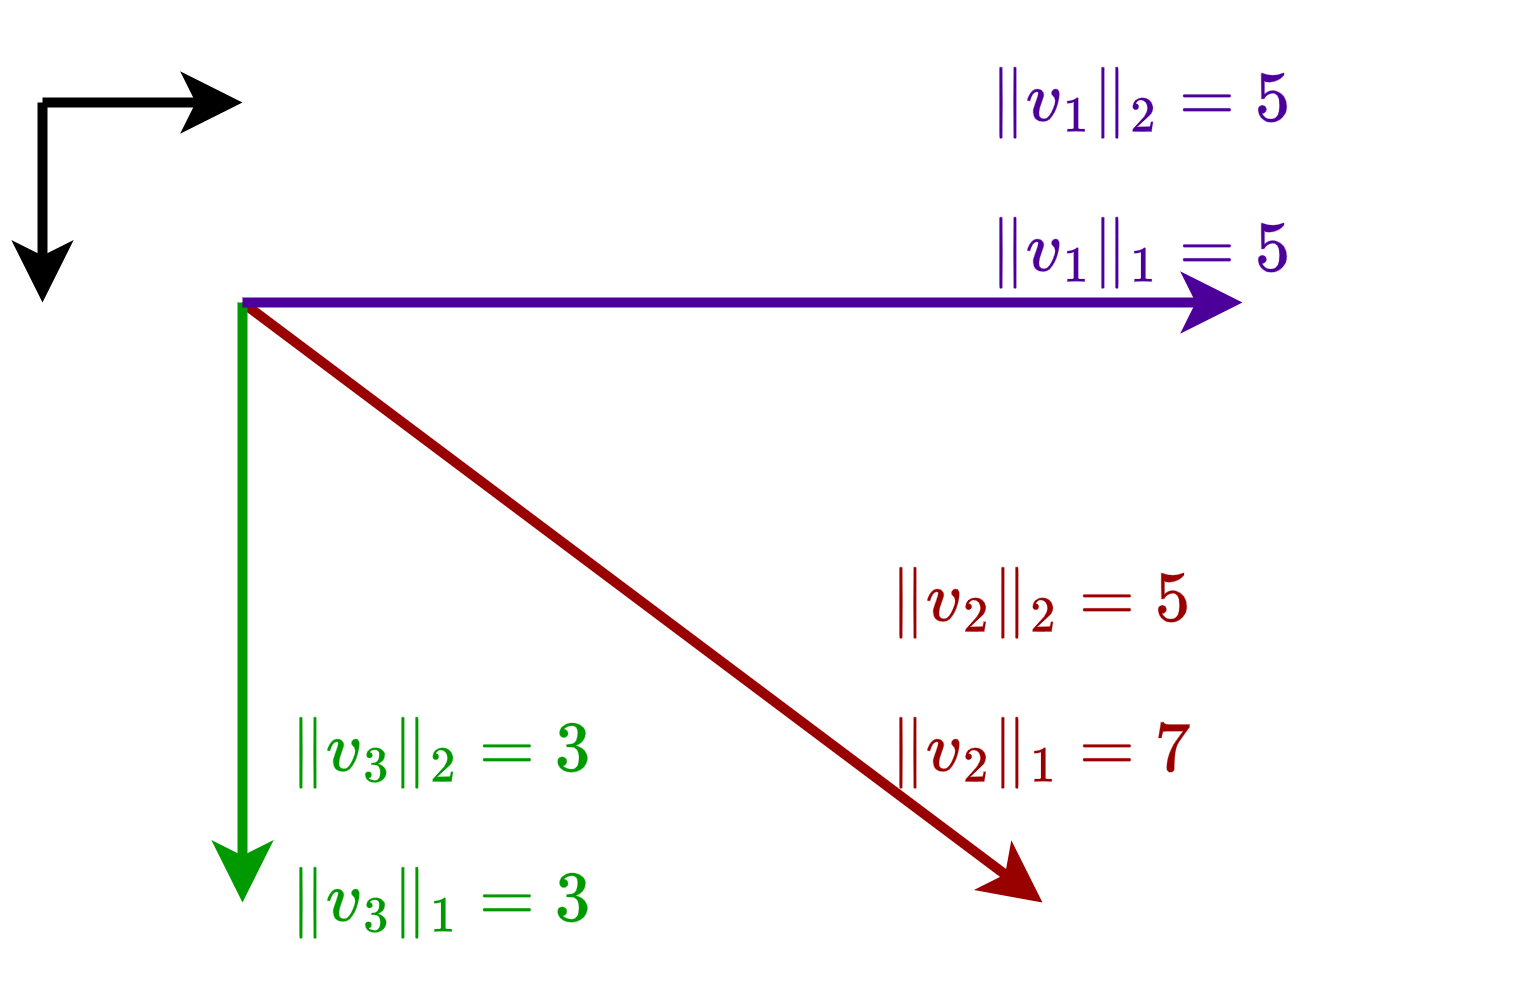
\includegraphics[width=0.5\linewidth]{figs/chap1/1 Norm Visualization.drawio.png}
    \caption{Visualization of 1-Norm of vectors. Notice that $v_1$ and $v_2$ have the same length of $5$, $v_2$ has a 1-Norm of $8$.}
    \label{fig:one norm visual}
\end{figure}

The result of the 1-Norm for the pitch optimization algorithm is that it attempts to remain in one of two regimes to maintain a minimized force load. 
In other words, the pitch controller prefers a state where all thrust is generated by either the vertical rotors or the forward rotor.
Using both rotor groups simultaneously increases the magnitude of the objective function more unfavorably than the use of just one group.


\subsection{Moment Control}
\label{sec:momentControl}

It is desirable to find the necessary input moment on the system, given the system model and current state. 
The pitch angle optimization function outputs a desired theta for each time step. 
The object of this section is to find the moment needed to actuate the system to achieve that particular pitch angle $\theta$ reference.

To derive this, the relationship between pitch moment $m$ and angular acceleration $\ddot{\theta}$, is given as

\begin{align*}
    \ddot{\theta} = \frac{1}{J_y} M
\end{align*}.

If there is a desired $\ddot{\theta}_{ref}$, then there is a corresponding desired $m_{des}$ given as

\begin{align}
  M_{des} = J_y \ddot{\theta}_{ref}
\end{align}.

This assumes that there is no error or disturbance in the system and that this controller tracks the desired pitch perfectly. 
However, this is unlikely, a proportional and derivative gain is attached to this equation, which yields

\begin{align}
    M_{des} = J_y \left(\ddot{\theta}_{ref} + k_d\left(\dot{\theta}_{ref} - q \right) + k_p\left(\theta_{ref} - \theta \right) \right)
\end{align}.

This relationship can be shown in a flowchart in Fig. \ref{fig:feedforwardThetaMoment}. 
Note that this does not yet relate to actuation controls.
Rather, it relates a desired pitch angle in a given moment of time to a desired moment to be generated by the state of the craft and by actuation.
In other words, the net moment that is desired to be controlled by the rotors and actuator is the output from this feedforward PID control.

\begin{figure}
    \centering
    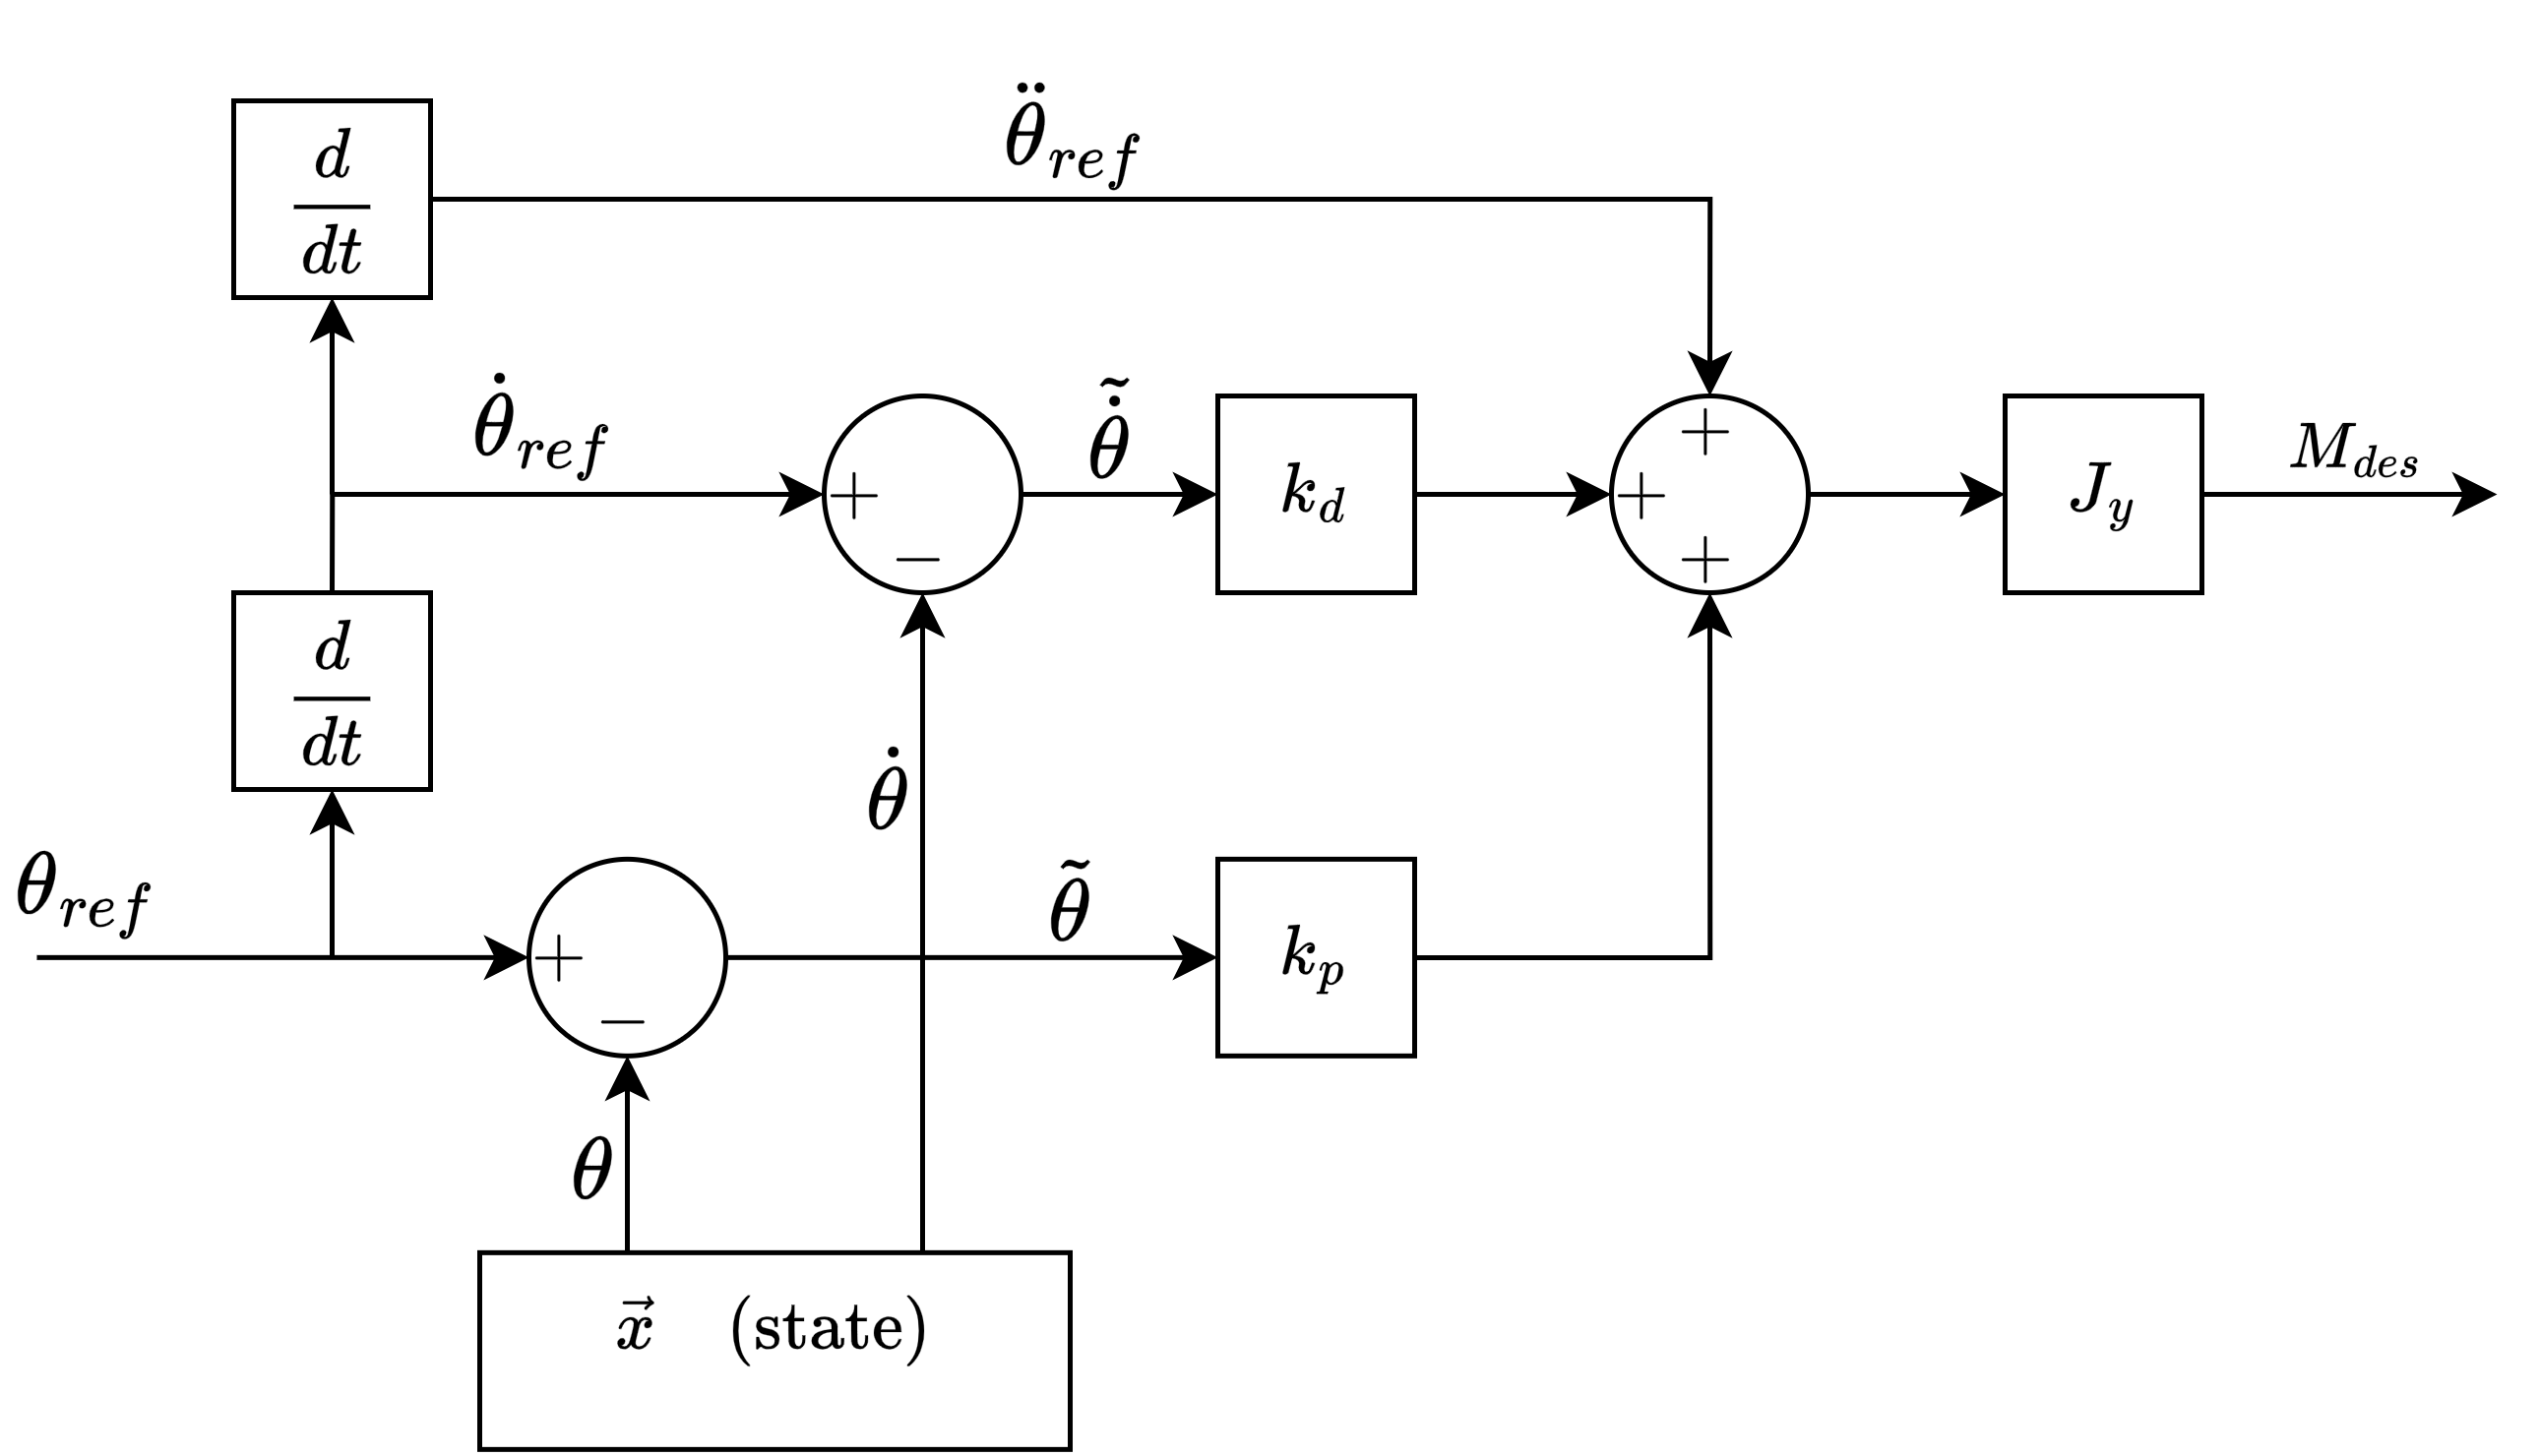
\includegraphics[width=0.75\linewidth]{figs/chap1/Moment Control Flowchart.drawio.png}
    \caption{Control Diagram between input $\theta_{ref}$ and output $M_{des}$.}
    \label{fig:feedforwardThetaMoment}
\end{figure}

\section{Elevator Control}

This autopilot is created to maximize the possible control authority due to the airspeed from the aircraft.
This was true for the residual desired force, and it is again true for desired moment.
The next task is to maximize control authority from elevator control, which minimizes needed moment control from the rotors.
The net aircraft moment may be expanded as

\begin{equation}
    M_{total} = M_0 + M_q q + M_{\delta_e} \delta_e + M_p
    \label{eq:MomentsSum}
\end{equation}.

where

\begin{align}
    \bar{q} = \frac{1}{2} \rho V_a^2\\
    \bar{q}_M = \bar{q} S c\\
    M_{aero} = \bar{q}_M \left[C_{M_0} + C_{M_{\alpha}} \alpha + C_{M_q} \frac{c}{2V_a} q + C_{M_{\delta_e}} \delta_e \right] \\
    M_0 = \bar{q}_M \left[C_{M_0} + C_{M_{\alpha}} \alpha \right]\\
    M_q = \bar{q}_M \left[ C_{M_q} \frac{c}{2V_a} \right]\\
    M_{\delta_e} = \bar{q}_M C_{M_{\delta_e}}\\
    M_p = l_f T(\delta_{t,f}) - l_r T(\delta_{t,r})
\end{align}.

Note that $M_0$ contains the airfoil coefficient, the $\alpha$ coefficient, and $\alpha$ itself, while $M_q$ and $M_{\delta_e}$ do not contain $q$ and $\delta_e$ respectively. 
$M_{total}$ is treated as the net moment on the quadplane and $M_{des}$ is treated as the desired net moment on the aircraft. 
The term $M_0$ represents the torque generated by the aircraft's current state including its angle of attack, airspeed, and characteristic shape. 
$M_q q$ represents the moment of the aircraft given the current pitch rate and $M_{\delta_e} \delta_e$ represents the moment given the current elevator control.
$M_p$ represents the moment caused by a differential vertical propeller control.

To maximize the pitch moment without the differential vertical rotors, the propeller term is initially set to zero as $M_p = 0$. 
This yields

\begin{align}
    \label{eq:momentsSum}
    M_{des} = M_0 + M_q q + M_{\delta_e} \delta_e + 0
\end{align}.

The only unknown in this equation is $\delta_e$.
The equation is then solved for $\delta_e$ as

\begin{align}
    \delta_e = \frac{M_{des} - M_0 - M_q q }{M_{\delta_e}}
\end{align}.

However, $\delta_e$ can only operate between values $[-\bar{\delta_e},\bar{\delta_e}]$, so this may become infeasible. 
A saturation value is created based on the set bounds for $\delta_e$.
The equation for $\delta_e$ is saturated as

\begin{align}
    \label{eq:saturateDeltaE}
    \delta_e^\ast = \text{sat}_{\Delta_e}\left(\frac{M_{des} - M_0 - M_q q}{M_{\delta_e}}\right) \\
    \Delta_e = [-\bar{\delta_e},\bar{\delta_e}]
\end{align}.

With this $\delta_e^\ast$, the desired propeller moment may be found by rearranging Eq. \ref{eq:MomentsSum} as

\begin{equation}
    M_p = M_{des} - M_0 - M_q q - M_{\delta_e} \delta_e^\ast
\end{equation}.

This is the desired moment that must be actuated by the vertical propellers, which is passed on to the rotor controller.

\section{Rotor Control}

Now with a desired vertical force, forward force, and pitch moment, the desired thrust from each of the three rotors is calculated.
These are: $T_t$, the forward propeller, $T_f$, the front vertical rotor, and $T_r$, the rear vertical rotor.

It is seen from the design of the quadplane in Fig. \ref{fig:quadplane_2D} that each of the three rotors generates forces directly on the $\hat{n}$ and $\hat{d}$ vectors of the body frame. 
The thrust vector for each rotor is given in the 2D body frame for front, rear, and forward thrusts as

\begin{align}
    \bs{F}_f(\delta_f) = 
    \begin{bmatrix}
        0\\
        -1\\
    \end{bmatrix}
    \space T(\delta_f)\\
    \bs{F}_r(\delta_r) = 
    \begin{bmatrix}
        0\\
        -1\\
    \end{bmatrix}
    \space T(\delta_r)\\
    \bs{F}_t(\delta_t) = 
    \begin{bmatrix}
        1\\
        0\\
    \end{bmatrix}
    \space T(\delta_t)
    \label{eq:thrustDirections}
\end{align}

The two vertical rotors (front and rear) generate thrust in the up, or negative down direction, while the forward rotor generates thrust in the positive north direction. 
This is rather convenient because the high level controller sets a desired force in the north (x) and down (z) direction.
Therefore, there is no mixing matrix required to map the rotor thrust directions to the body frame axes.

The desired propeller force vector may be decomposed as 

\begin{align}
    \bs{F}^b_{p,des} =
    \begin{bmatrix}
        \bs{F}^b_{p,des,x}\\
        \bs{F}^b_{p,des,z}
    \end{bmatrix}
\end{align}.

$\bs{F}^b_{p,des,x}$ was defined as the force desired in the positive $x$ direction of the aircraft, and was calculated in the pitch optimization section \ref{sec:PitchOptimization}.
The only force that acts in the positive $x$ direction is the forward rotor, so the desired force in the $x$ direction is defined as the desired thrust from the forward propeller as

\begin{equation}
    T_{t,des} = \bs{F}^b_{p,des,x}
\end{equation}.

It is assumed in this paper that the relationship between rotor thrust and control input is linear.
The thrust for the forward thruster, given the control input $\delta_t$ is then $T(\delta_t) = T_{max} \cdot \delta_t$.
By rearranging this equation, the control input for forward thrust is given as

\begin{equation}
    \delta_{t,des} = \frac{T_{des}}{T_{max}}
\end{equation}.


$\bs{F}^b_{p,des,z}$ is the residual desired force in the $z$ direction. 
This produces two equations which are functions of the two vertical rotors $T_{f}$ and $T_{r}$ as

\begin{align}
    \bs{F}^b_{p,des,z} = -T_f(\delta_f) - T_r(\delta_r)\\
    M_p = T_f(\delta_f) l_f - T_r(\delta_r) l_r
\end{align}.

There are now two equations and two unknowns in a linear relationship. This may be arranged as

\begin{align}
    \begin{bmatrix}
        \bs{F}^b_{p,des,z}\\
        M_p\\
    \end{bmatrix}
    =
    \begin{bmatrix}
        -1 & -1\\
        l_f & -l_r\\
    \end{bmatrix}
    \begin{bmatrix}
        T_f(\delta_f)\\
        T_r(\delta_r)\\
    \end{bmatrix}
\end{align}

The solution for all three rotor thrusts then becomes

\begin{align}
    \begin{bmatrix}
        T_f(\delta_f)\\
        T_r(\delta_r)\\
    \end{bmatrix}
    =
    \begin{bmatrix}
        -1 & -1\\
        l_f & -l_r\\
    \end{bmatrix}^{-1}
    \begin{bmatrix}
        \bs{F}^b_{p,des,z}\\
        M_p\\
    \end{bmatrix}\\
    T_t(\delta_t) = \bs{F}^b_{p,des,x}
\end{align}.

The $\delta$ control input for each of these thrusts is obtained as

\begin{align}
    \delta_{f,unsat} = \frac{T_{f,des}}{T_{max}}\\
    \delta_{r,unsat} = \frac{T_{r,des}}{T_{max}}\\
    \delta_{t,unsat} = \frac{T_{t,des}}{T_{max}}\\
\end{align}.

Then, each control input is saturated to stay within the bounds of: $0 \leq \delta_{throttle} \leq 1$ as

\begin{align}
    \delta_f = sat(\delta_{f,unsat})\\
    \delta_r = sat(\delta_{r,unsat})\\
    \delta_t = sat(\delta_{t,unsat})\\
\end{align}.

\subsection{Review of Controller}

The controller described in the previous sections is somewhat complicated, and it may be difficult to follow. 
Similar controllers in the literature are often called daisy chain or cascaded controllers.
Fig. \ref{fig:ControllerOverview} 
details the several stages of the controller. 
The two inputs are the reference trajectory $p_{ref}(t)$ and the quadplane state $x$.

The pitch free trajectory tracker finds the desired net force to be actuated on the aircraft $F_{des}^i$, after taking into account state error $\tilde{x}$, gravity $g e_z$, and reference acceleration $\ddot{p}_{ref}(t)$.
It does so using a state error gain matrix $K$, which is set using LQR.

Pitch optimization finds the optimal pitch $\theta$ that minimizes the 1 norm error between desired force and aerodynamic force on the airframe.
This finds the pitch that generates the largest possible lift from the airframe before rotor actuation is taken into account.
Pitch optimization also finds the residual force $F^b_{p,des}$ that is necessary to be generated by the three quadplane rotors $\delta_t, \delta_f, \delta_r$.

Moment control finds the desired pitch moment to be actuated on the aircraft.
The second derivative of desired pitch $\theta$ input from pitch optimization is taken as $\ddot{\theta}$, or angular acceleration.
If no pitch error $\tilde{\theta}$ or pitch rate error $\dot{\tilde{\theta}}$ exists, then the the desired moment is the angular acceleration $\ddot{\theta}$ times rotational inertia about the pitch axis $J_y$.
If $\tilde{\theta}$ or $\dot{\tilde{\theta}}$ are nonzero, then they are added to net angular acceleration using proportional and derivative gains.

The elevator controller finds the elevator control $\delta_e$ to get net desired moment from moment control; this minimizes the moment that must be generated by the vertical rotors.
Elevator controller is saturated to within elevator range $\left[-\bar{\delta_e}, \bar{\delta_e}\right]$

Rotor control allocation finds the control inputs to generate the remaining forces $F^b_{p,des}$ and moment $M_{des}$.

\begin{figure}
    \centering
    \includegraphics[width=0.85\linewidth]{figs/chap1/controllerOverview.jpg}
    \caption{Overview of VTOL controller. Divided into five main sections. 1. Pitch free trajectory tracker, 2. Pitch optimization, 3. Moment control, 4. Elevator Control, 5. Rotor control allocation.}
    \label{fig:ControllerOverview}
\end{figure}


\section{Path Planning}
\label{sec:vtol path planning}

A particularly difficult problem here is that a path needs to be created which provides a smooth transition from vertical hovering to forward flight. 
This requires a path that goes from an initial vertical velocity to a horizontal velocity. 
It is desirable to have a gradual acceleration from vertical takeoff velocity of around $1 \frac{m}{s}$ to a forward airspeed of $25 \frac{m}{s}$. 
To do this, a flight path was developed in the shape of root functions, including a $2^{nd}, 3^{rd},$ and $4^{th}$ root shapes. 
As the flight path progressed, the spacing gradually increased to meet the initial and final conditions.

This required calculating the arc length of a section of the polynomial. 
The simplest method for creating these curves was through parametric equations given as $n(t)$ representing the north position, and $a(t)$ representing the altitude. 
The general form of arc length for the curve is

\begin{align}
    L = \int_a^b \sqrt{\left(\frac{d \space n(t)}{dt}\right)^2 + \left(\frac{d \space a(t)}{dt}\right)^2}
\end{align}.

This is computed numerically, and split up to gradually increase the spacing of control points to provide continuous increase of desired velocity.

\subsection{Flight Path Shape}

It is necessary to develop a useful flight path for the VTOL. 
One might ask what shape of path provides a lower energy consumption while also providing stability.
One possibility is a square root flight path, where the VTOL starts at the vertex in vertical lift-off mode, and slowly transitions into a forward trajectory. 
At some point, the slope is close enough to flat to justify transition to forward flight.

\subsection{Root Flight Path}

It is desirable to create a flight path for the eVTOL to follow between a vertical takeoff and forward flight. 
A well-behaved function shape for a takeoff or landing is a square root function, which is defined as

\begin{align}
    f(x) = A(B(x-x_0))^\frac{1}{2} + a_0\\
    \frac{\partial f}{\partial x} = \frac{AB}{2}(B(x-x_0))^{-\frac{1}{2}}
\end{align}.

In order to generalize the square root function to more easily take the derivative, the parametric equation is defined as

\begin{align}
    n(t) = \frac{t^2}{B} + n_0\\
    a(t) = At + a_0\\
\end{align}.

The parametric derivative of that function is given as

\begin{align}
    n(t) = \frac{t^2}{B} + n_0\\
    \frac{\partial a(t)}{\partial n(t)} = \frac{AB}{2t}
\end{align}.

The variable $t$ in this equation is not the actual trajectory time, but is the parameter needed to for the parametric equation. 
$A$ and $B$ are vertical and horizontal scalars for the equations, and $n_0$ and $a_0$ represent the starting north and altitude positions respectively.

\section{Controller Tuning}

\subsection{LQR Tuning}
This controller contrains two sets of tunable parameters. 
The $K$ gain matrix from the pitch-free trajectory tracking, and the $p$ and $d$ gains from the moment control section.
Recall from section \ref{sec:PitchFree} that $K$ must be selected for $\tilde{\bs{u}}_F^i = -K \tilde{\bs{x}}^i$.
For an LQR controller, $Q$ and $R$ matrices must be selected. 
In this realization, an integrator term was included as well. 
For the results that follow, these were selected as

\begin{align}
    P_{err,max} = 10.0\\
    p = \frac{1}{P_{err,max}^2}\\
    V_{err,max} = 1.0\\
    v = \frac{1}{V_{err,max}^2}\\
    I_{max} = 5.0\\
    i = \frac{1}{I_{max}^2}\\
    Q = \mathrm{diag}(p,p,v,v,i,i)\\
    R = diag(1.0, 1.0)\\
\end{align}.

$K$ and $k_i$ were then selected using the python control library LQR function.

\subsection{Feedforward Control Tuning}

In subsection \ref{sec:momentControl} the control law for desired moment is

\begin{align}
    m_{des} = J_y \left(\ddot{\theta}_{ref} + k_d\left(\dot{\theta}_{ref} - q \right) + k_p\left(\theta_{ref} - \theta \right) \right)
\end{align}.

In this case, $k_p$ and $k_d$ were selected using rise time $t_r$ and damping coefficient $\zeta$ as

\begin{align}
    \omega_n = \frac{\pi}{2 t_r \sqrt{1 - \zeta^2}}\\
    k_p = \frac{\omega_n^2}{J_y}
    k_d = \frac{2 \zeta \omega_n}{J_y}
\end{align}.

In this case $t_r = 2.0$ and $\zeta = 0.707$.

\section{Results}

A 2D quadplane dynamic system was simulated to test and prove the viability of this controller. 
A dynamic 2D quadplane model was developed in a Python repository using the equations of motion given in this chapter. 
This dynamic system uses the Runge-Kutte algorithm to propagate dynamic systems described by systems of differential equations.

For this implementation, the coeffecients of aerodynamics are set forth in table \ref{tb:vtolCoefficients}.
\begin{table}
\label{tb:vtolCoefficients}
\centering
\caption{Aerodynamic Coefficients for VTOL}
\begin{tabular}{|c c !{\vrule width 1.2pt} c c !{\vrule width 1.2pt} c c|}
    \hline
    $C_{L_0}$ & 0.23 & $C_{D_0}$ & 0.0424 & $C_{M_0}$ & 0.0135\\
    \hline
    $C_{L_\alpha}$ & 5.61 & $C_{D_\alpha}$ & 0.132 & $C_{M_\alpha}$ & -2.74\\
    \hline
    $C_{L_q}$ & 7.95 & $C_{D_q}$ & 0.0 & $C_{M_q}$ & -38.21\\
    \hline
    $C_{L_{\delta_e}}$ & 0.13 & $C_{D_{\delta_e}}$ & 0.0135 & $C_{M_{\delta_e}}$ & -0.99\\
    \hline
\end{tabular}
\end{table}

To test this controller, several flight paths were created and tested. 
Their results, including position and velocity errors, and the attached videos are presented in the following sections.

\subsubsection{A Note On Initial and Final Conditions}

There are two sets of boundary conditions that must be satisfied in order for the aircraft to successfully complete this trajectory. 
For a degree 3 B-Spline, the position, velocity, and acceleration at both start and end must both be defined. 
These are the initial and final conditions of the trajectory.

When the aircraft is at start, its position is at the origin, for this particular problem. 
It is given a very small initial velocity, like it just barely took off. 
It may also be given a small vertical acceleration.
These initial conditions are represented as

\begin{align}
    \bs{S} = 
    \begin{bmatrix}
        \bs(p)(0) & \frac{d\bs{p}}{dt}(0) & \frac{d^2 \bs{p}}{dt^2}(0)
    \end{bmatrix}
    =
    \begin{bmatrix}
        0.0 & 0.0 & 0.0\\
        0.0 & -0.1 & 0.0\\
    \end{bmatrix}
\end{align}.

When the aircraft is at the end of the trajectory, it is $500$ meters north at an altitude of $100$ meters, with a forward airspeed of $25.0$ meters per second, and zero acceleration. 
This takes place at time $M$, and is shown mathematically as

\begin{align}
    \bs{E} = 
    \begin{bmatrix}
        \bs(p)(M) & \frac{d\bs{p}}{dt}(M) & \frac{d^2 \bs{p}}{dt^2}(M)
    \end{bmatrix}
    =
    \begin{bmatrix}
        500 & 25 & 0\\
        -100 & 0 & 0\\
    \end{bmatrix}
\end{align}.

Three precisely placed control points satisfy each set of three conditions. 
The relationship between sets of conditions and control points developed more in Chapter \ref{ch:BSplines}, but the direct relationships are given as

\begin{align}
    \bs{C}_{1:3} = S (\hat{B}_M^2(0))^{-1}
\end{align}

and

\begin{align}
    \bs{C}_{M-d:M} = E (\hat{B}_M^2(M))^{-1}
\end{align}.

This obtains three start and three end control points, as shown in Fig. \ref{fig:startEndControlPoints}.

\begin{figure}[htbp]
    \centering
    \begin{subfigure}{0.48\textwidth}
        \centering
        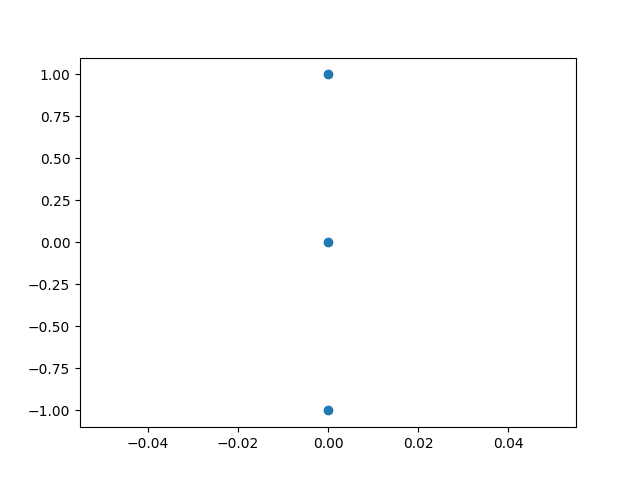
\includegraphics[width=\linewidth]{figs/chap1/Takeoff/startControlPoints.png}
        \caption{Three evenly spaced initial control points for the trajectory with an initial velocity of 0.1.}
        \label{fig:startControlPoints}
    \end{subfigure}
    \hfill
    \begin{subfigure}{0.48\textwidth}
        \centering
        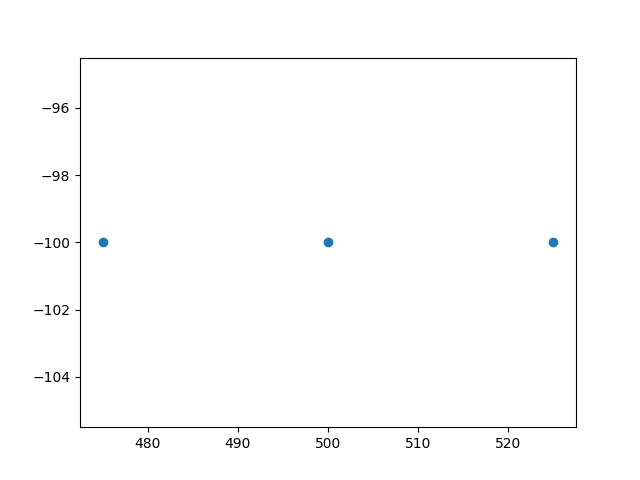
\includegraphics[width=\linewidth]{figs/chap1/Takeoff/endControlPoints.png}
        \caption{Three evenly spaced final control points for the trajectory with a final velocity of 25.}
        \label{fig:endControlPoints}
    \end{subfigure} 

    \begin{subfigure}{1.0\textwidth}
        \centering
        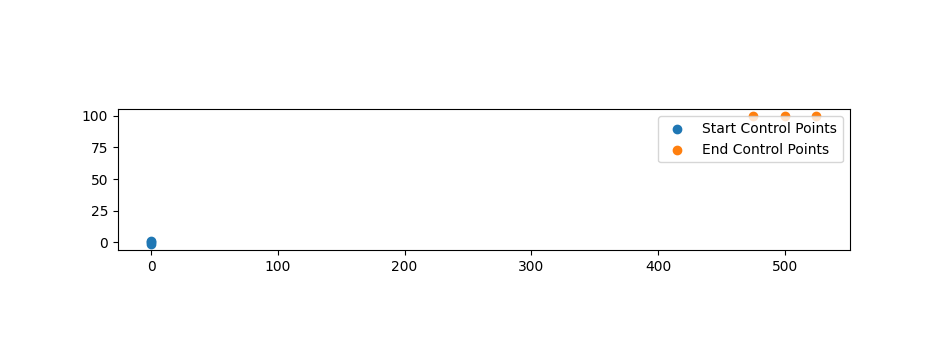
\includegraphics[width=\linewidth]{figs/chap1/Takeoff/startEndControlPoints_2.png}
        \caption{Initial and final control points for trajectory.}
        \label{fig:startAndEndControlPoints}
    \end{subfigure} 

    \caption{}
    \label{fig:startEndControlPoints}
\end{figure}


Now that these initial and final conditions are set, the intervening control points may be generated. 
The final start control $C_3$ point is set as the apex of the square root function, and the first end control point $C_{M-d}$ is set as the final position. 
The spacing between control points $C_2$ and $C_3$ as $C_3 - C_2$ becomes the start spacing.
The spacing between control points $C_{M-d}$ and $C_{M-d+1}$ as $C_{M-d+1} - C_{M-d}$ are the final spacing of control points. 
Along the trajectory, each successive control point is placed so that there is smooth change of spacing.
This is done so that there is a relatively constant acceleration between start and finish.

\subsection{Takeoff}

The first segment of flight is takeoff. 
It is desirable to find a way to take the aircraft into the air and begin its path before transitioning to full fixed-wing flight. 
To do this, an the square root function trajectory was generated as $y=\sqrt{x}$. 
That is, the spatial shape of the trajectory is a sampled square root function, and shown in Fig. \ref{fig:TakeoffShape}.

\begin{figure}[htbp]
    \centering
    \begin{subfigure}{1.0\textwidth}
        \centering
        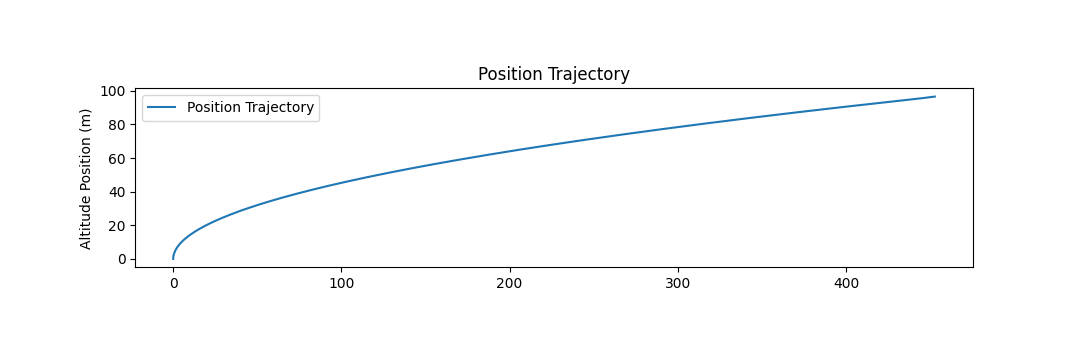
\includegraphics[width=\linewidth]{figs/chap1/Takeoff/Takeoff shape without control points.png}
        \caption{Takeoff positional trajectory. Plots altitude with respect to north position, moving from left to right.}
        \label{fig:TakeoffShapeNoControl}
    \end{subfigure}
    
    \begin{subfigure}{1.0\textwidth}
        \centering
        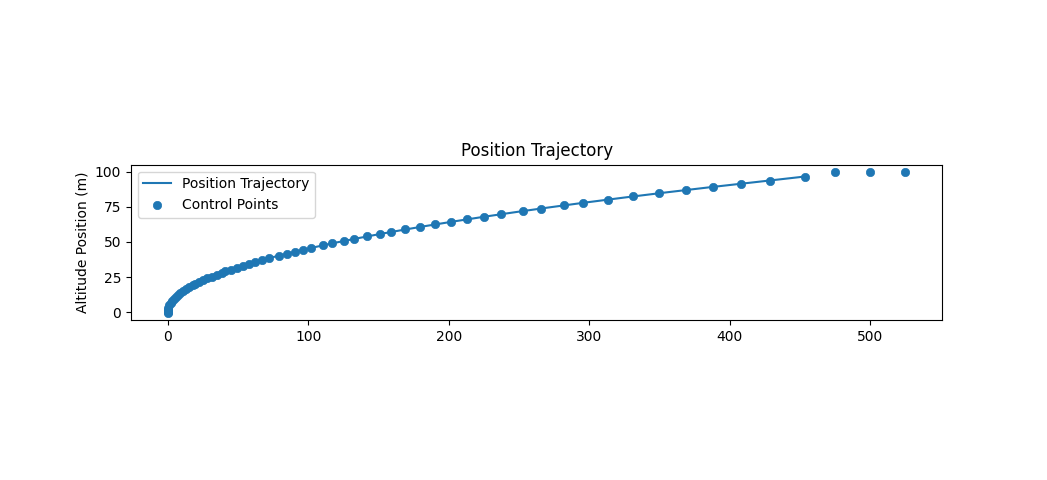
\includegraphics[width=\linewidth]{figs/chap1/Takeoff/Takeoff shape with control points.png}
        \caption{Takeoff positional trajectory. Plots altitude with respect to north position. Includes control points in diagram.}
        \label{fig:TakeoffShapeWithControl}
    \end{subfigure}
    \caption{Plots of takeoff shape. Path found using scaled function of $d = -\sqrt{n}$. The control points, shown in subfigure \ref{fig:TakeoffShapeWithControl}, are spaced increasingly far apart to simulate increasing velocity.}
    \label{fig:TakeoffShape}
\end{figure}

The square root function was selected because at time $t=0$, the immediate direction of the B-Spline is directly vertical, which corresponds to vertical take off, and then a nearly level section, which corresponds to forward flight.

This flight path was loaded into the controller, and the following results were collected. 
A video of this flight path is viewable at \href{https://youtu.be/pRFlPvZbulI}{https://youtu.be/pRFlPvZbulI}. 
The figures showing metrics for this controller are shown at \ref{fig:TakeoffMetrics}.

\begin{figure}[htbp]
    \centering
    \begin{subfigure}{0.48\textwidth}
        \centering
        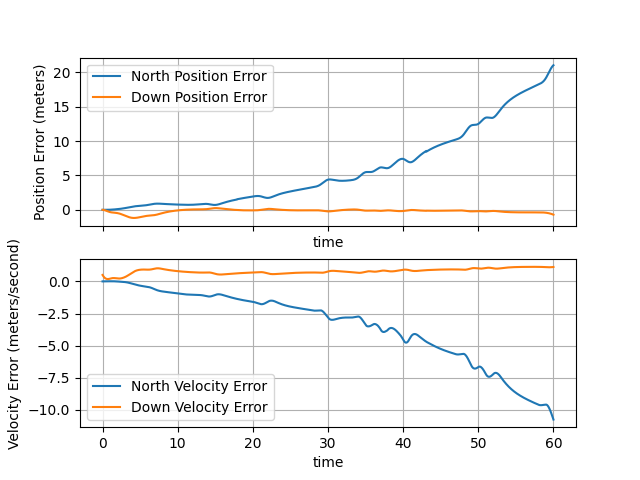
\includegraphics[width=\linewidth]{figs/chap1/Takeoff/posVelError.png}
        \caption{Position and velocity errors in both north and down directions over takeoff trajectory.}
        \label{fig:TakeoffPosVelError}
    \end{subfigure}
    \hfill
    \begin{subfigure}{0.48\textwidth}
        \centering
        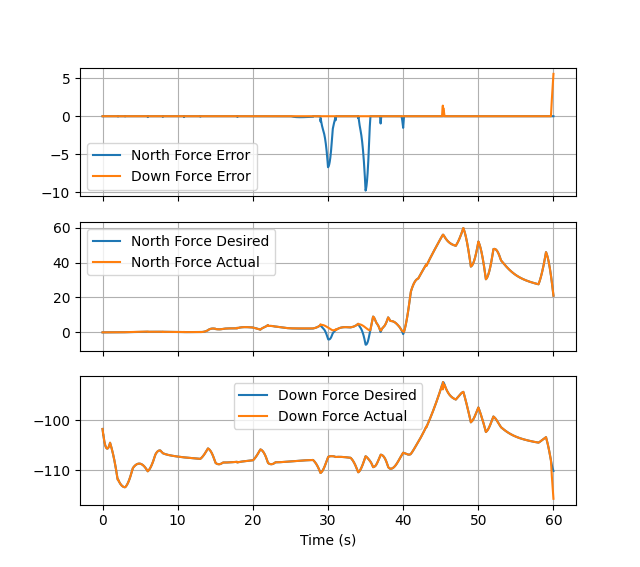
\includegraphics[width=\linewidth]{figs/chap1/Takeoff/ForcesComparison.png}
        \caption{Compares actual and desired forces and the error between them.}
        \label{fig:TakeoffForceComparison}
    \end{subfigure}

    \vspace{0.5cm}  % vertical spacing between rows

    % Row 2
    \begin{subfigure}{1.0\textwidth}
        \centering
        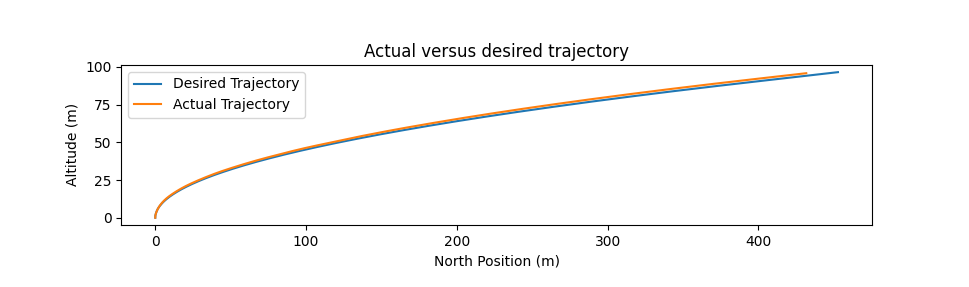
\includegraphics[width=\linewidth]{figs/chap1/Takeoff/TrajectorActualAndDesired.png}
        \caption{Comparison of the actual trajectory versus desired trajectory.}
        \label{fig:TakeoffVelComparison}
    \end{subfigure}
    \hfill
    \vspace{0.5cm}  % vertical spacing between rows

    % Row 2
    \begin{subfigure}{0.48\textwidth}
        \centering
        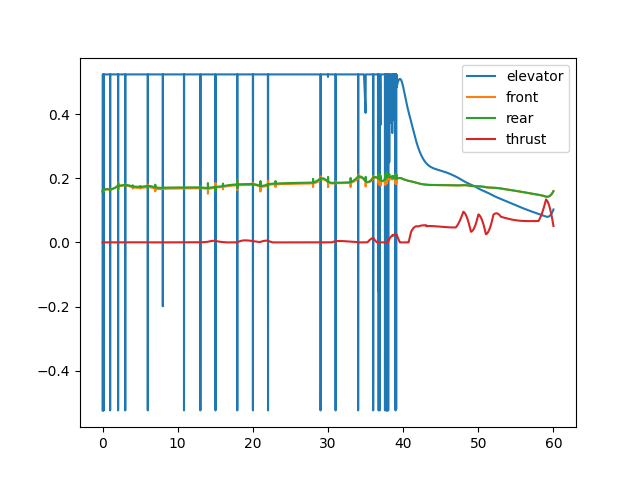
\includegraphics[width=\linewidth]{figs/chap1/Takeoff/Deltas.png}
        \caption{Deltas control inputs for the controller over the entire trajectory. Notice that at the transition point, the elevator begins to modulate and not simply saturate at its maximum value.}
        \label{fig:TakeoffDeltas}
    \end{subfigure}
    \hfill
    \begin{subfigure}{0.48\textwidth}
        \centering
        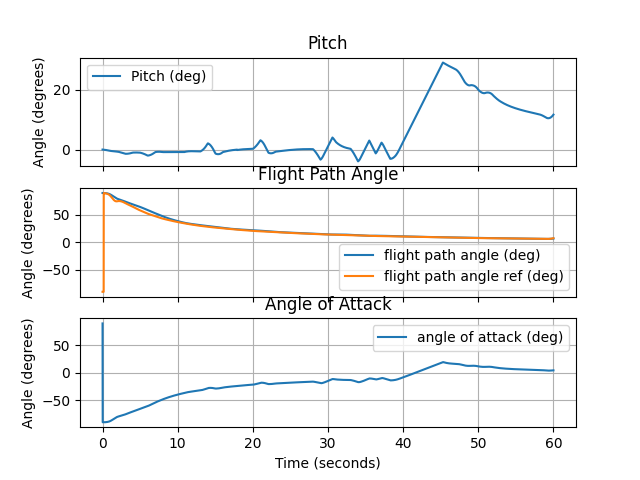
\includegraphics[width=\linewidth]{figs/chap1/Takeoff/Angles.png}
        \caption{Pitch, flight path angle, and angle of attack for the aircraft through takeoff trajectory.}
        \label{fig:TakeoffAngles}
    \end{subfigure}    
    \label{fig:TakeoffMetrics}
    \caption{Takeoff metrics and plots}
\end{figure}


\subsection{Takeoff and Forward Flight}

After the takeoff segment has been flown by the aircraft, the flight path may transition to a straight forward segment.
In this test, the takeoff segment was identical to the previous segment, but a long segment for straight forward flight was also connected.
That is, the control points were placed for a reference trajectory of $25 \frac{m}{s}$.
The metrics for this controller are shown in Fig. \ref{fig:TransitionMetrics}.

\begin{figure}[htbp]
    \centering
    \begin{subfigure}{0.48\textwidth}
        \centering
        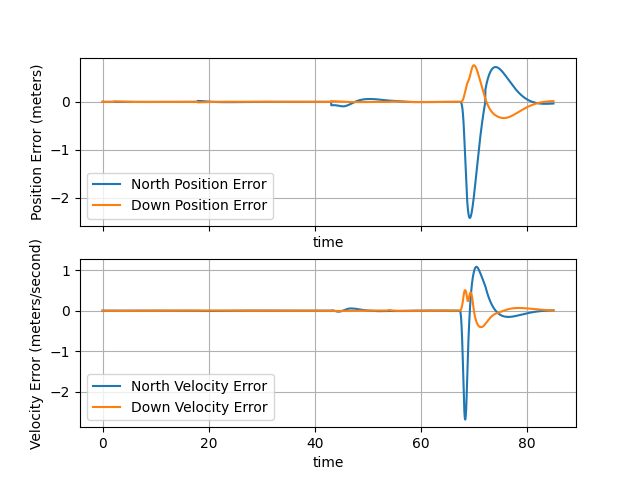
\includegraphics[width=\linewidth]{figs/chap1/complete_path/PosVelErrors.png}
        \caption{Position and velocity errors in both north and down directions over takeoff trajectory.}
        \label{fig:TransitionPosVelError}
    \end{subfigure}
    \hfill
    \begin{subfigure}{0.48\textwidth}
        \centering
        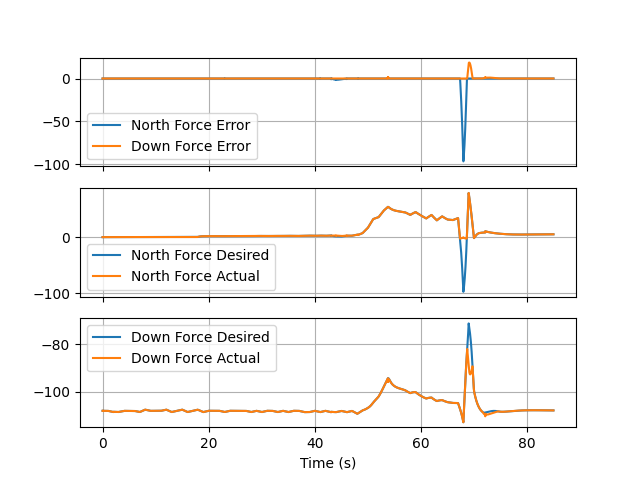
\includegraphics[width=\linewidth]{figs/chap1/complete_path/forceErrors.png}
        \caption{Compares actual and desired forces and the error between them.}
        \label{fig:TransitionForceComparison}
    \end{subfigure}

    \vspace{0.5cm}  % vertical spacing between rows

    % Row 2
    \begin{subfigure}{1.0\textwidth}
        \centering
        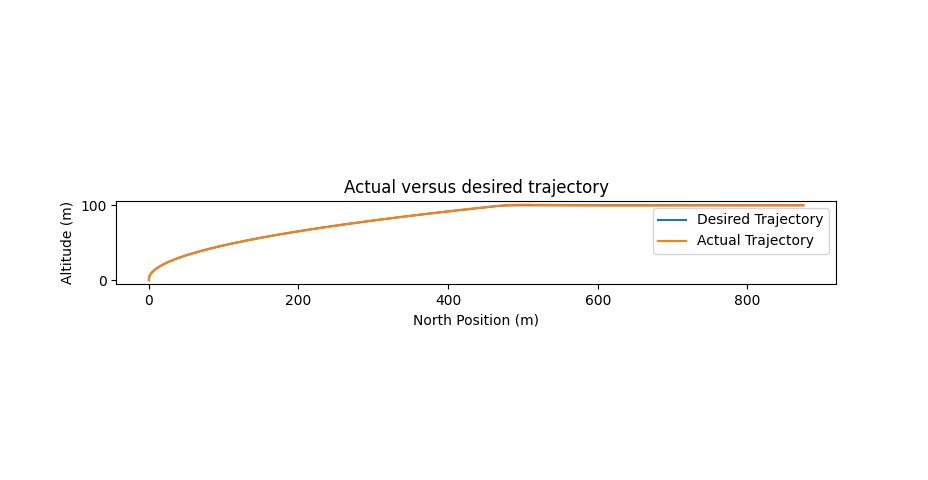
\includegraphics[width=\linewidth]{figs/chap1/complete_path/trajectory_comparisons.png}
        \caption{Comparison of the actual trajectory versus desired trajectory.}
        \label{fig:TransitionVelComparison}
    \end{subfigure}
    \hfill
    \vspace{0.5cm}  % vertical spacing between rows

    % Row 2
    \begin{subfigure}{0.48\textwidth}
        \centering
        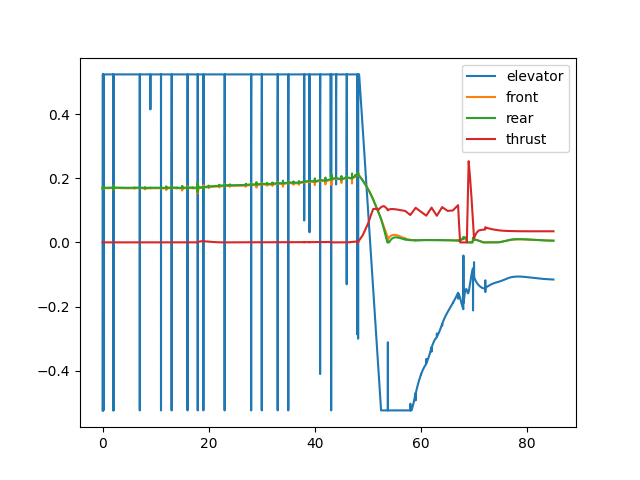
\includegraphics[width=\linewidth]{figs/chap1/complete_path/Deltas.png}
        \caption{Deltas control inputs for the controller over the entire trajectory.}
        \label{fig:TransitionDeltas}
    \end{subfigure}
    \hfill
    \begin{subfigure}{0.48\textwidth}
        \centering
        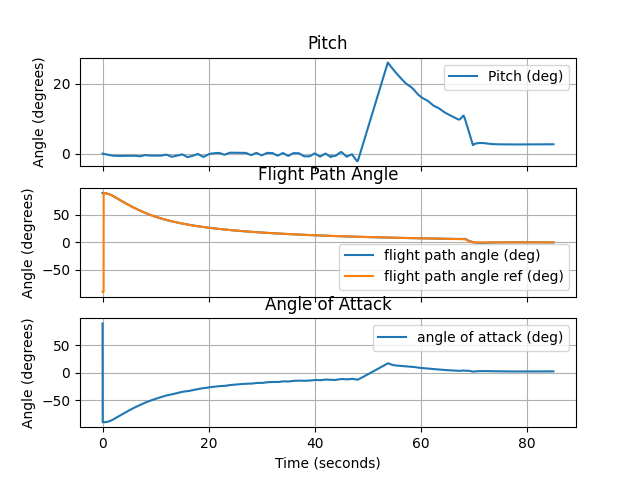
\includegraphics[width=\linewidth]{figs/chap1/complete_path/angles.png}
        \caption{Pitch, flight path angle, and angle of attack for the aircraft through takeoff trajectory.}
        \label{fig:TransitionAngles}
    \end{subfigure}    
    \label{fig:TransitionMetrics}
    \caption{Transition metrics and plots}
\end{figure}


\subsection{Landing}
\label{sec:landing}

In order for this aircraft controller to be a viable solution, the aircraft must land. 
A trajectory very similar to the takeoff trajectory was constructed, except in the opposite direction. 
The start and end conditions are reversed along with the direction of the square root function as

\begin{align}
    \bs{S} =
    \begin{bmatrix}
        \bs(p)(0) & \frac{d\bs{p}}{dt}(0) & \frac{d^2 \bs{p}}{dt^2}(0)
    \end{bmatrix}
    =
    \begin{bmatrix}
        0 & 25 & 0\\
        -100 & 0 & 0\\
    \end{bmatrix}\\
    \bs{E} =
    \begin{bmatrix}
        \bs(p)(M) & \frac{d\bs{p}}{dt}(M) & \frac{d^2 \bs{p}}{dt^2}(M)
    \end{bmatrix}
    =
    \begin{bmatrix}
        500.0 & 0.0 & 0.0\\
        0.0 & -0.1 & 0.0\\
    \end{bmatrix}
\end{align}.

This produces the trajectory in Fig. \ref{fig:LandingTrajectory}.

\begin{figure}
    \centering
    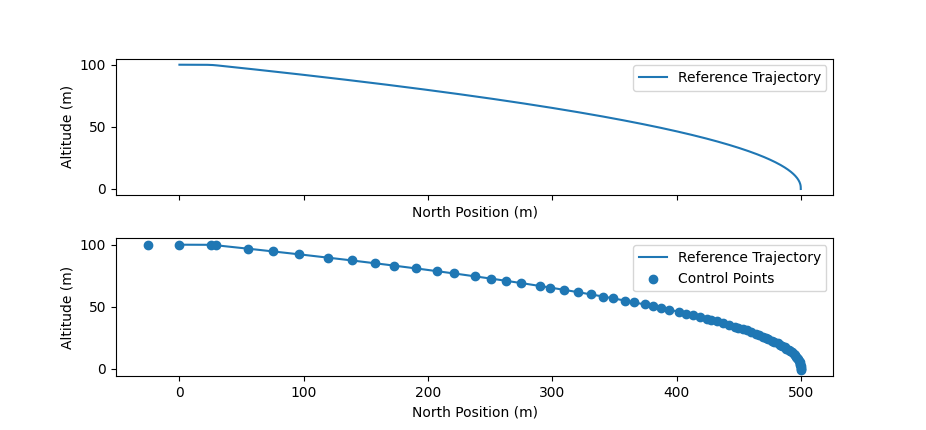
\includegraphics[width=0.7\linewidth]{figs/chap1/landing/ReferenceTrajectory.png}
    \caption{Landing trajectory both with and without control points, with an initial velocity of $25 \frac{m}{s}$ and altitude of $100 m$, and landing $500$ meters north.}
    \label{fig:LandingTrajectory}
\end{figure}

In simulation, the aircraft is started with the same conditions as the trajectory, which is velocity of $25 \frac{m}{s}$ and altitude of $100 m$. A video of this manuever may be found at \href{https://youtu.be/w4bYAqHPQaI}{https://youtu.be/w4bYAqHPQaI}, and metrics for the controller are shown in Fig. \ref{fig:LandingMetrics}


\begin{figure}[htbp]
    \centering
    \begin{subfigure}{0.48\textwidth}
        \centering
        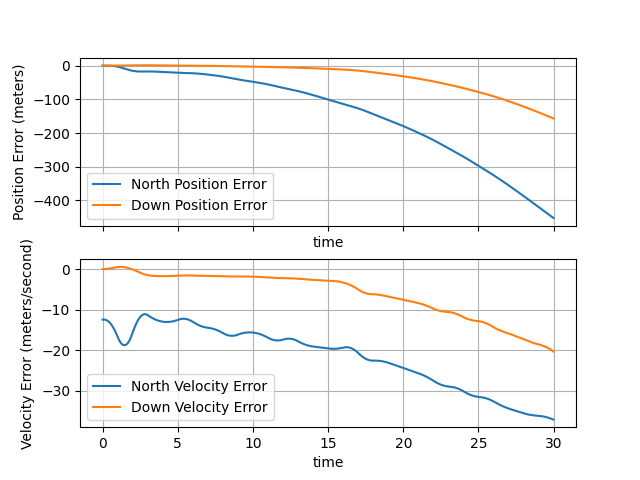
\includegraphics[width=\linewidth]{figs/chap1/landing/PosVelErrors.png}
        \caption{Position and velocity errors in both north and down directions over landing trajectory.}
        \label{fig:LandingPosVelError}
    \end{subfigure}
    \hfill
    \begin{subfigure}{0.48\textwidth}
        \centering
        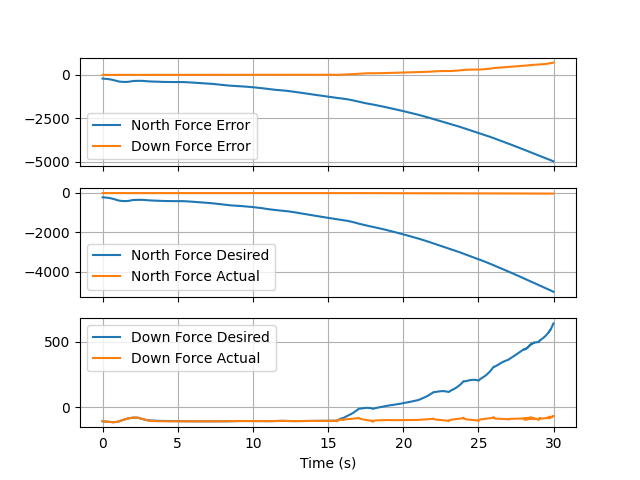
\includegraphics[width=\linewidth]{figs/chap1/landing/ForcesComparisons.png}
        \caption{Compares actual and desired forces and the error between them.}
        \label{fig:LandingForceComparison}
    \end{subfigure}

    \vspace{0.5cm}  % vertical spacing between rows

    % Row 2
    \begin{subfigure}{1.0\textwidth}
        \centering
        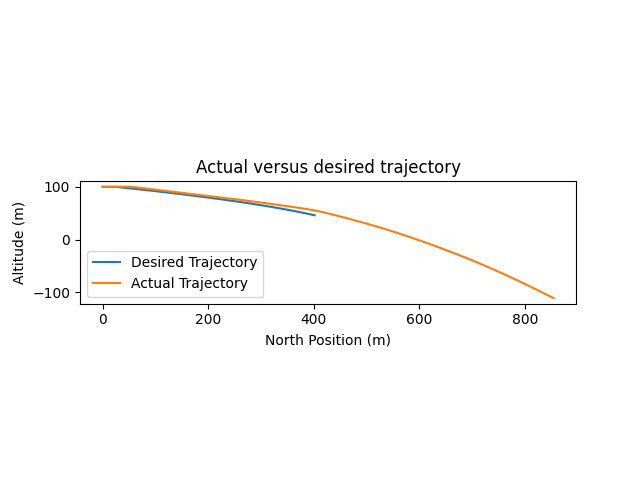
\includegraphics[width=\linewidth]{figs/chap1/landing/DesiredActualTrajectory.png}
        \caption{Comparison of the actual trajectory versus desired trajectory.}
        \label{fig:LandingVelComparison}
    \end{subfigure}
    \hfill
    \vspace{0.5cm}  % vertical spacing between rows

    % Row 2
    \begin{subfigure}{0.48\textwidth}
        \centering
        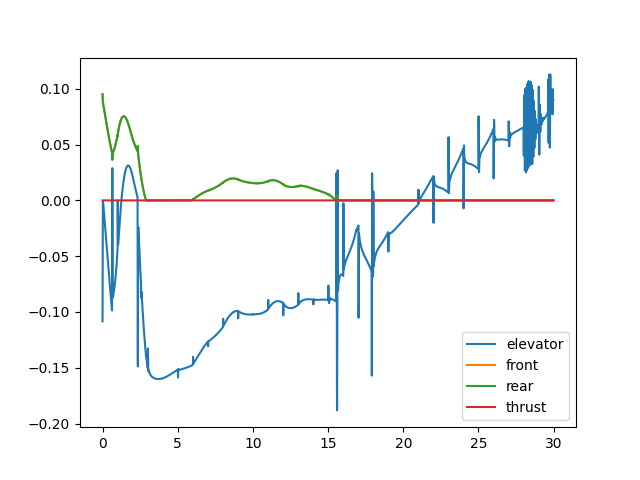
\includegraphics[width=\linewidth]{figs/chap1/landing/Deltas.png}
        \caption{Deltas control inputs for the controller.}
        \label{fig:LandingDeltas}
    \end{subfigure}
    \hfill
    \begin{subfigure}{0.48\textwidth}
        \centering
        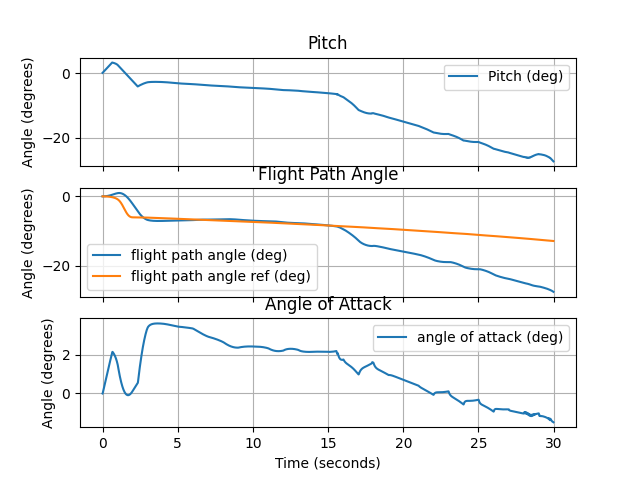
\includegraphics[width=\linewidth]{figs/chap1/landing/Angles.png}
        \caption{Pitch, flight path angle, and angle of attack for the aircraft through landing trajectory.}
        \label{fig:LandingAngles}
    \end{subfigure}    
    \label{fig:LandingMetrics}
    \caption{Landing metrics and plots}
\end{figure}

In this case, it is immediately obvious that the aircraft does not follow the desired trajectory. Instead of slowing down and closely tracking the trajectory, the aircraft does not slow down, but keeps going forward at relatively the same velocity. 
This phenomenon is discussed in more detail in the future work section. 
If the trajectory requires a negative force, or negative acceleration, in the body frame north direction, the aircraft is unable to follow it.

\subsection{Successive Ascent}

Another test for the autopilot is with a series increasing slopes to test whether the aircraft can track those inputs. 
An example of this framework is shown in Fig. \ref{fig:successiveAscent}. 
In this flight path, each section has a larger flight path angle $\gamma$ than the previous one. 
In this test, the sections go $0^{\circ}$, $10^{\circ}$, $20^{\circ}$, $30^{\circ}$ respectively, with the same north spacing of $400$ meters for each segment. 

\begin{figure}
    \centering
    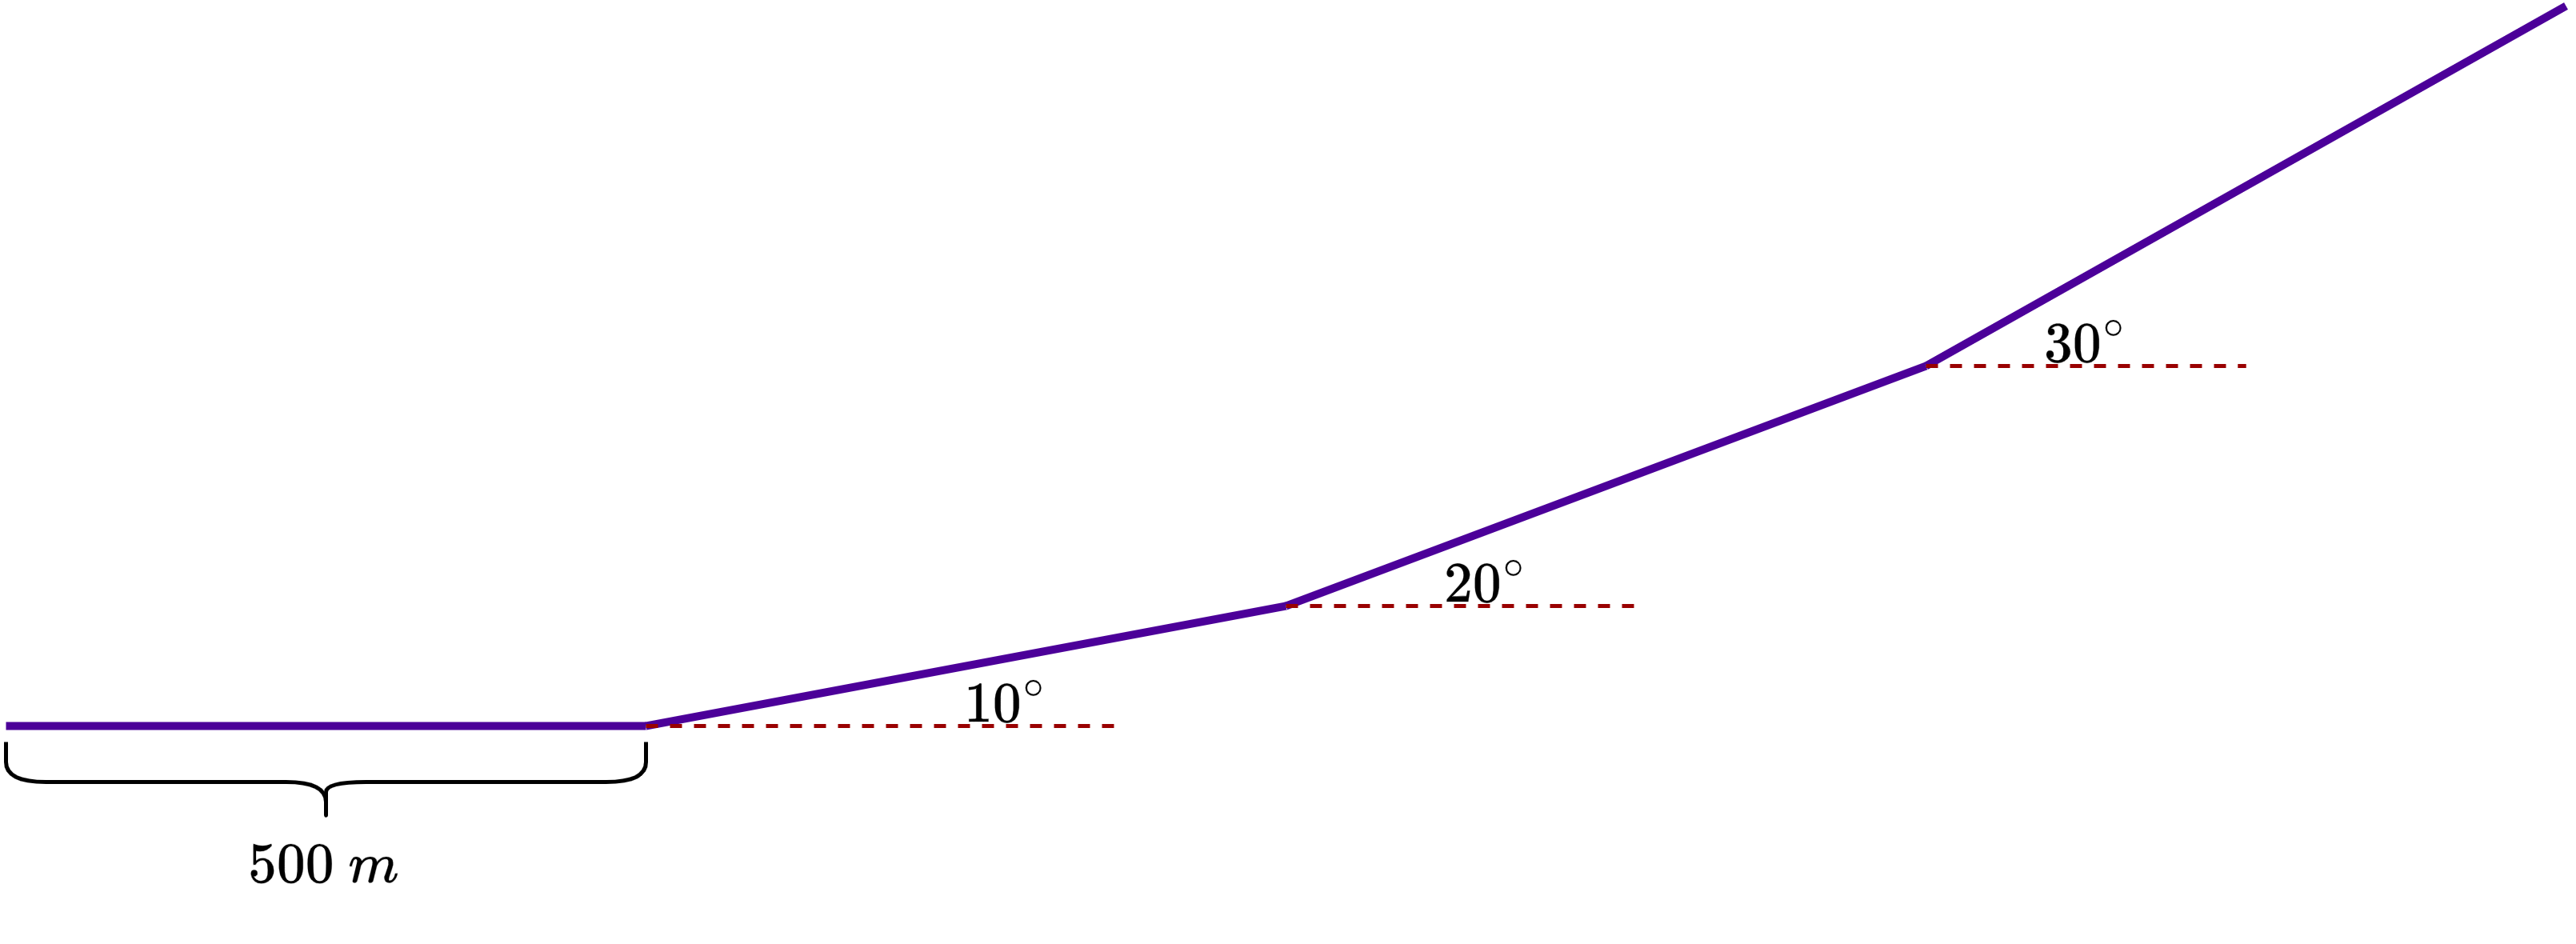
\includegraphics[width=0.7\linewidth]{figs/chap1/successiveAscent/Successive Ascent.drawio.png}
    \caption{Example of successive ascent flight path, where each segment has a north length of $400$ meters. Each segment has a path angle $\gamma$ of $0^{\circ}$, $10^{\circ}$, $20^{\circ}$, and $30^{\circ}$ respectively.}
    \label{fig:successiveAscent}
\end{figure}

In this case, the aircraft starts out level, with an initial north velocity of $V_n = 25.0 \frac{m}{s}$. 
This diagram shows the lines along which control points are placed. 
The actual trajectory smooths out the corners somewhat.
The control points are spaced in a manner such that the reference velocity remains $25.0 \frac{m}{s}$ for the entire trajectory. 
A full video of the simulation is available at \href{https://youtu.be/-ZMKCkmkpCI}{Successive Ascent Video}.

\begin{figure}[htbp]
    \centering
    \begin{subfigure}{0.48\textwidth}
        \centering
        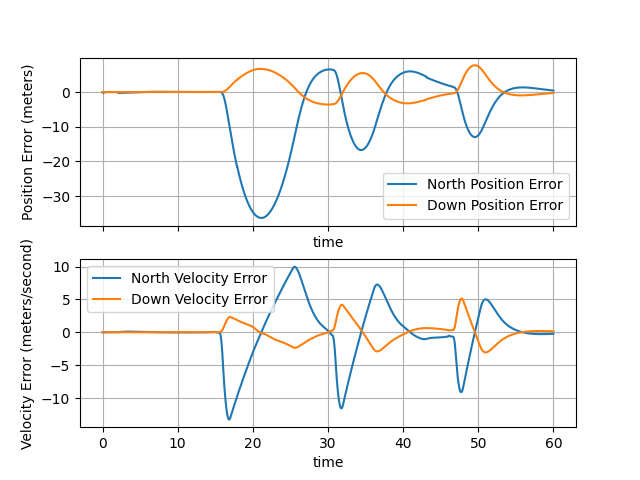
\includegraphics[width=\linewidth]{figs/chap1/successiveAscent/PosVelErrors.png}
        \caption{Position and velocity errors in both north and down directions over successive ascent trajectory.}
        \label{fig:SuccessivePosVelError}
    \end{subfigure}
    \hfill
    \begin{subfigure}{0.48\textwidth}
        \centering
        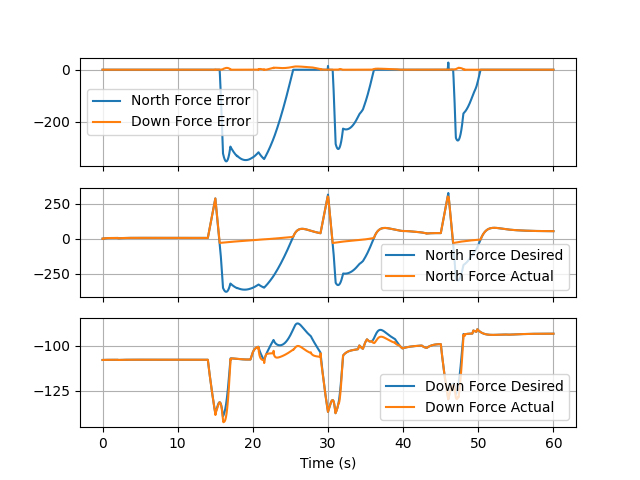
\includegraphics[width=\linewidth]{figs/chap1/successiveAscent/forceComparisons.png}
        \caption{Compares actual and desired forces and the error between them.}
        \label{fig:SuccessivePosComparison}
    \end{subfigure}

    \vspace{0.5cm}  % vertical spacing between rows

    % Row 2
    \begin{subfigure}{1.0\textwidth}
        \centering
        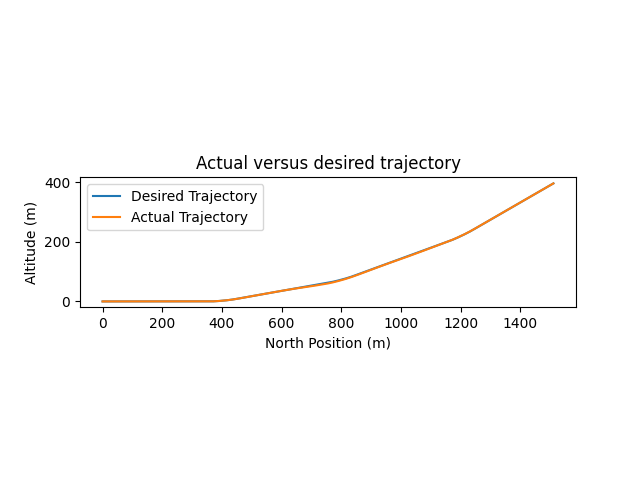
\includegraphics[width=\linewidth]{figs/chap1/successiveAscent/TrajectoryComparisons.png}
        \caption{Comparison of the actual trajectory versus desired trajectory.}
        \label{fig:SuccessiveTrajComparison}
    \end{subfigure}
    \hfill
    \vspace{0.5cm}  % vertical spacing between rows

    % Row 2
    \begin{subfigure}{0.48\textwidth}
        \centering
        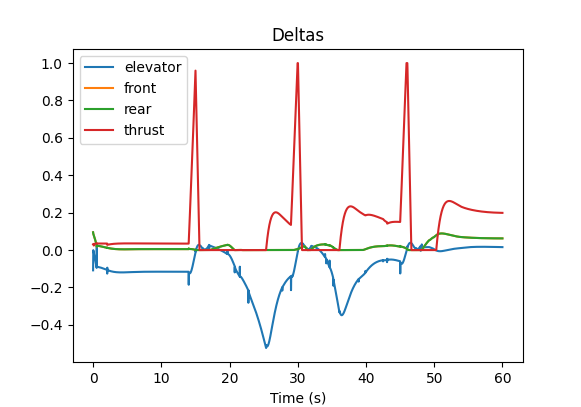
\includegraphics[width=\linewidth]{figs/chap1/successiveAscent/Deltas.png}
        \caption{Deltas control inputs for the controller.}
        \label{fig:SuccessiveDeltas}
    \end{subfigure}
    \hfill
    \begin{subfigure}{0.48\textwidth}
        \centering
        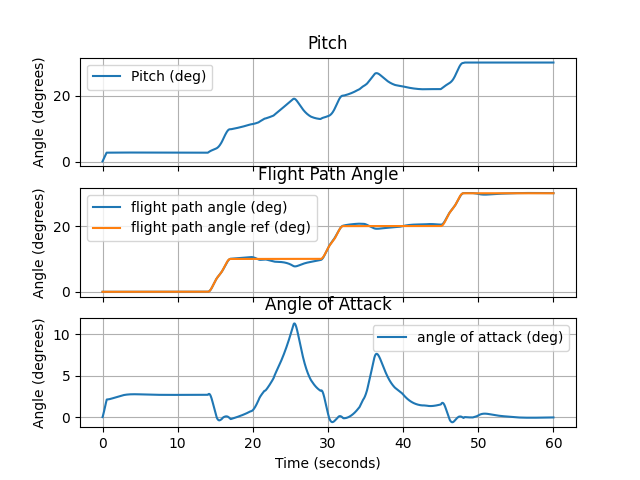
\includegraphics[width=\linewidth]{figs/chap1/successiveAscent/angles.png}
        \caption{Pitch, flight path angle, and angle of attack for the aircraft through successive ascent trajectory.}
        \label{fig:SuccessiveAngles}
    \end{subfigure}    
    \label{fig:SuccessiveMetrics}
    \caption{Successive ascent metrics and plots.}
\end{figure}

In these successively steeper flight paths, the aircraft was successfully able to track the trajectory. 
As the angle gets progressively steeper, the vertical propellers have to do more work to keep the aircraft on trajectory.

Notice from Fig. \ref{fig:SuccessiveVelComparison} that the actual velocities approach the desired velocities, but don't quite get there until the end of each segment.
For the velocity, this is an underdamped controller.  
This may be tuned in the future for better performance.

\begin{figure}
    \centering
    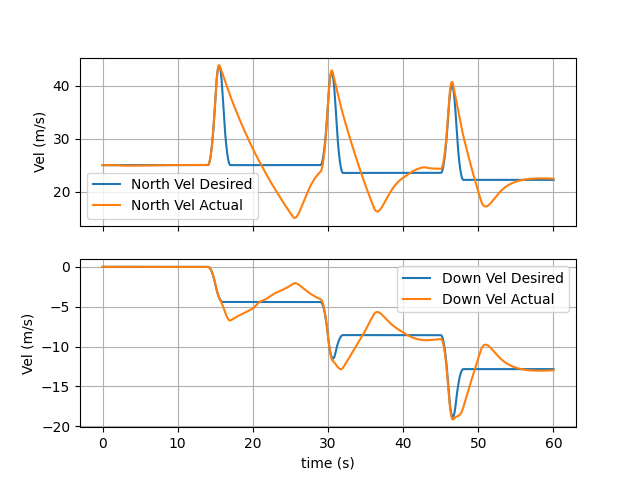
\includegraphics[width=\linewidth]{figs/chap1/successiveAscent/VelocitiesComparisons.png}
    \caption{Comparison of desired versus actual velocities in the north and down directions for successive ascent.}
    \label{fig:SuccessiveVelComparison}
\end{figure}

\subsection{Step Convergence}

The autopilot should also be subject to tests against error, to determine if the aircraft can converge to a trajectory when it does not start directly on the desired trajectory.
A test was constructed with the forward input trajectory at a constant forward velocity of $25 \frac{m}{s}$.
The altitude of the trajectory was $0$.
The aircraft started with an initial altitude of $-25$ meters, and an initial forward velocity of $25 \frac{m}{s}$.
This is the equivalent of a step input reference to the system for altitude. 
The metrics for this experiment are shown in Fig. \ref{fig:StepMetrics}, and the video for this experiment is found at \href{https://youtu.be/AVDS21xf7JI}{https://youtu.be/AVDS21xf7JI}. 


\begin{figure}[htbp]
    \centering
    \begin{subfigure}{0.48\textwidth}
        \centering
        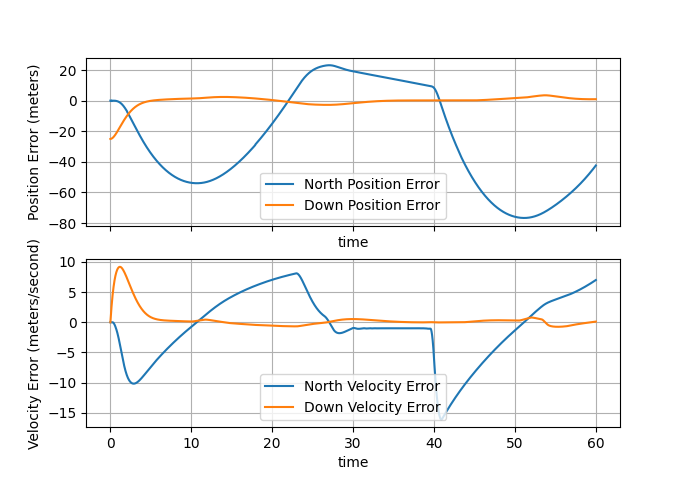
\includegraphics[width=\linewidth]{figs/chap1/StepError/PosVelErrors.png}
        \caption{Position and velocity errors in both north and down directions over successive ascent trajectory.}
        \label{fig:StepPosVelError}
    \end{subfigure}
    \hfill
    \begin{subfigure}{0.48\textwidth}
        \centering
        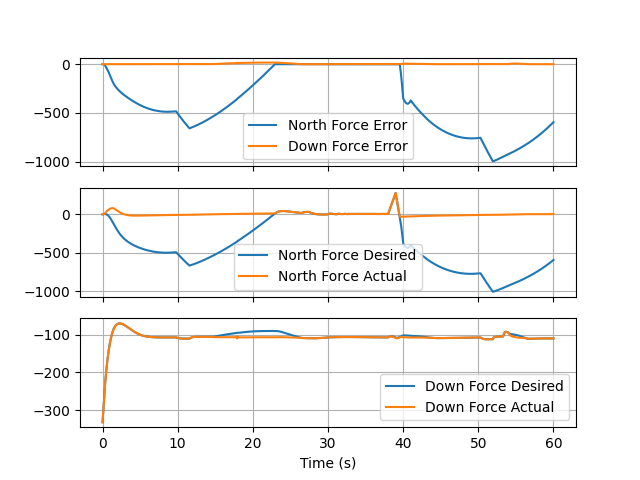
\includegraphics[width=\linewidth]{figs/chap1/StepError/forcesComparison.png}
        \caption{Compares actual and desired forces and the error between them.}
        \label{fig:StepForcesComparison}
    \end{subfigure}

    \vspace{0.5cm}  % vertical spacing between rows

    % Row 2
    \begin{subfigure}{0.48\textwidth}
        \centering
        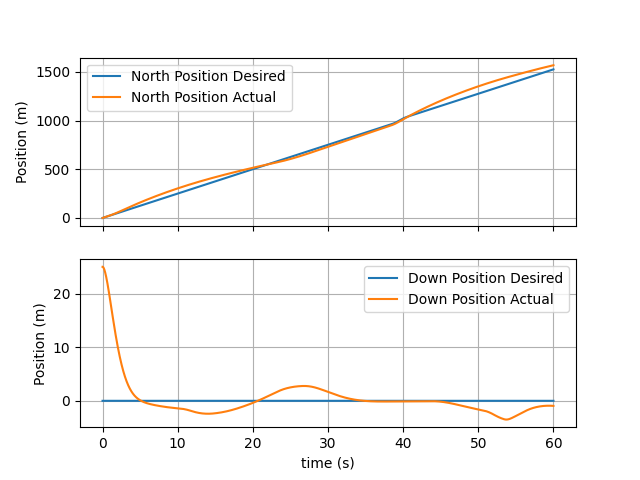
\includegraphics[width=\linewidth]{figs/chap1/StepError/PosComparisons.png}
        \caption{Comparison of the actual position versus desired position.}
        \label{fig:StepPosComparison}
    \end{subfigure}
    \hfill
    \begin{subfigure}{0.48\textwidth}
        \centering
        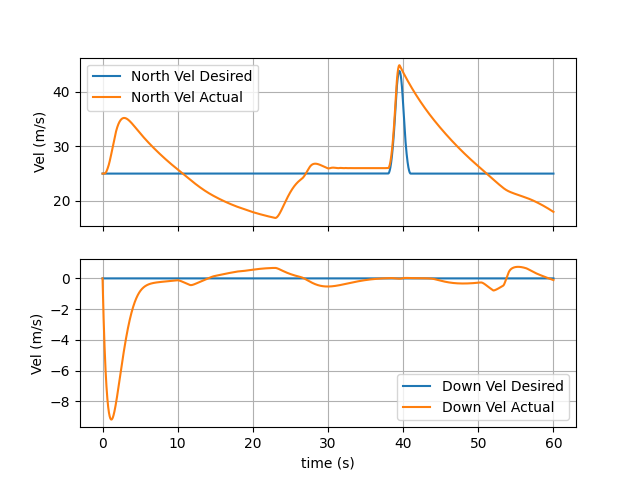
\includegraphics[width=\linewidth]{figs/chap1/StepError/VelComparisons.png}
        \caption{Comparison of the actual velocity versus desired velocity.}
        \label{fig:StepVelComparison}
    \end{subfigure}
    \hfill
    \vspace{0.5cm}  % vertical spacing between rows

    % Row 2
    \begin{subfigure}{0.48\textwidth}
        \centering
        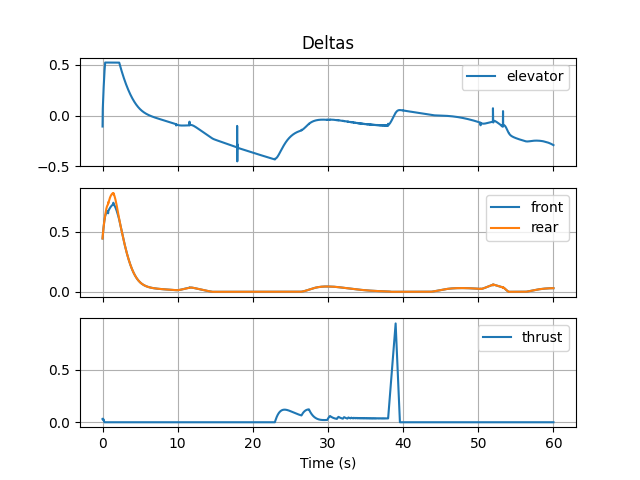
\includegraphics[width=\linewidth]{figs/chap1/StepError/Deltas2.png}
        \caption{Deltas control inputs for the controller.}
        \label{fig:StepDeltas}
    \end{subfigure}
    \hfill
    \begin{subfigure}{0.48\textwidth}
        \centering
        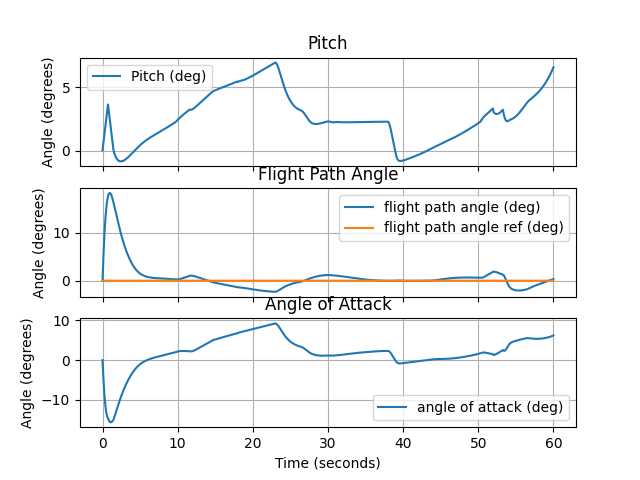
\includegraphics[width=\linewidth]{figs/chap1/StepError/angles.png}
        \caption{Pitch, flight path angle, and angle of attack for the aircraft through successive ascent trajectory.}
        \label{fig:StepAngles}
    \end{subfigure}    
    \label{fig:StepMetrics}
    \caption{Step metrics and plots.}
\end{figure}

In Fig. \ref{fig:StepMetrics}, the aircraft oscillates between north position and north velocity errors as it attempts to converge. 
This issue can be fixed in the future with better tuning.

\section{Current Issues and Future Work}

In its present state, this autopilot is only partially completed.
Significant improvement must be made before it can be successfully implemented on an actual hardware VTOL. 
The following are some considerations for challenges which must be overcome for a complete solution.

\subsection{Landing and Negative North Forces}

The biggest issue with trajectory tracking for the aircraft is apparent during landing. 
During the landing segment, the aircraft is required to slow down in the body frame north direction.
Therefore, the reference force in the body frame $n$ direction is negative.
When this happens, the control allocator attempts to allocate that negative thrust to the forward rotor, where a negative force means a negative desired thrust.
However, the aircraft cannot do this due to saturation constraints; this aircraft does not have unlimited actuation capacities, and most small UAVs do not have reverse thrust capacities.
From Equation \ref{eq:thrustDirections}, the thrust generated by the forward thruster is given in 3D and 2D by

\begin{align}
    \bs{F}^{3D}_t(\delta_t) = 
    \begin{bmatrix}
        1\\
        0\\
        0\\
    \end{bmatrix}
    \space T(\delta_t)
    \qquad
    \bs{F}^{2D}_t(\delta_t) = 
    \begin{bmatrix}
        1\\
        0\\
    \end{bmatrix}
    \space T(\delta_t)  
\end{align}.

And recall that $T(\delta_t)$ can only assume a value in the range

\begin{align}
    0 \leq T(\delta_t) \leq T_{max}
\end{align}.

This constrains the achievable thrust to be a positive value. 
If the desired force in the north body direction from the forward thruster, after taking into account aerodynamic and gravitational forces, is negative there is no mechanism in the aircraft to achieve this outcome. 
Therefore, the aircraft diverges from its desired trajectory. 
This is demonstrated as

\begin{align}
    \bs{F}^b_{p,des,x} < 0\\
    T_{t,des} = \bs{F}^b_{p,des,x}\\
    \delta_{t,unsat} = \frac{T_{des}}{T_{max}}, \quad \delta_{t,unsat} < 0\\
    \delta_t = sat(\delta_{t,unsat}), \quad \delta_t = 0
\end{align}.

\subsection{Safety Mechanisms}

With the increasing use of small unmanned aircraft, it becomes more important to have autopilot safety mechanisms in place. 
It is necessary to have default autopilots in place in case of a failure of an experimental autopilot, such as the one described in this paper. 
This is important for the case where the aircraft is not physically able to track a particular trajectory, as described in the above section. 
Future implementations of this autopilot must include safety parameters to revert back to a standard quadrotor or fixed-wing autopilot if things get out of hand.

\subsection{Model Uncertainty}

Perhaps the largest deficiency in this model and controller is its lack of robust and adaptive control. 
That is, this controller is entirely model dependent, and any discrepancy between the model causes the aircraft to become unstable.
In the case of this 2D model, this is especially true for lift and drag due to angle of attack during the transition phase.
In the future, this will require both aerodynamic estimation and a robust control strategy to deal with inevitable model deficiencies.

\subsection{3D Implementation}

Before this controller can be implemented in hardware, it must be generalized to a 3D model. 
This work originally started with a 3D model, with an initial attempt at model inversion. 
However, this proved unstable at the time and had to be temporarily abandoned for the 2D model.
A 3D implementation of the quadplane would include movement in the east $\hat{e}$ direction, roll $\phi$ about the $\hat{n}$ axis, and yaw $\psi$ about the $\hat{d}$ axis. 
This model would also include four vertical rotors, instead of two, ailerons $\delta_a$, and rudder $\delta_r$.
It must be demonstrated that this 3D model is differentially flat. 
Doing so will allow for the development of a 3D trajectory tracking controller, coupled $\phi$, $\theta$, and $\psi$ controllers, and a 3D dynamically inverting low level controller.
When this is completed, hardware implementation may move forward.

\subsection{Hardware}

Although this 2D quadplane controller is not ready for hardware testing, much hardware development has already taken place in this research group. 
Unfortunately, VTOL aircraft are currently a somewhat niche product. 
Even quadplanes tend to cost an order of magnitude more than their airplane and quadcopter counterpart, and often do not include replaceable parts. 
For these reasons, the research team has invested heavily in 3D printing airframes, specifically quadplane VTOL airframes. 
In the event of a crash that partially destroys a section of the airplane, that section can be reprinted and replaced quickly and cheaply.
By 3D printing aircraft, the research group is able to make custom modifications and additions to airframes, such as lidar mounts, weathervanes, and payloads.
This is done using foaming filaments, such as HT-LW PLA and ASA Aero.
Though 3D printing work extends to development of standard fixed-wing aircraft and quadrotor frames, the first fully functional 3D printed airframe has been a quadplane VTOL, as shown in Fig. \ref{fig:quadplane3DPrinted}.

\begin{figure}
    \centering
    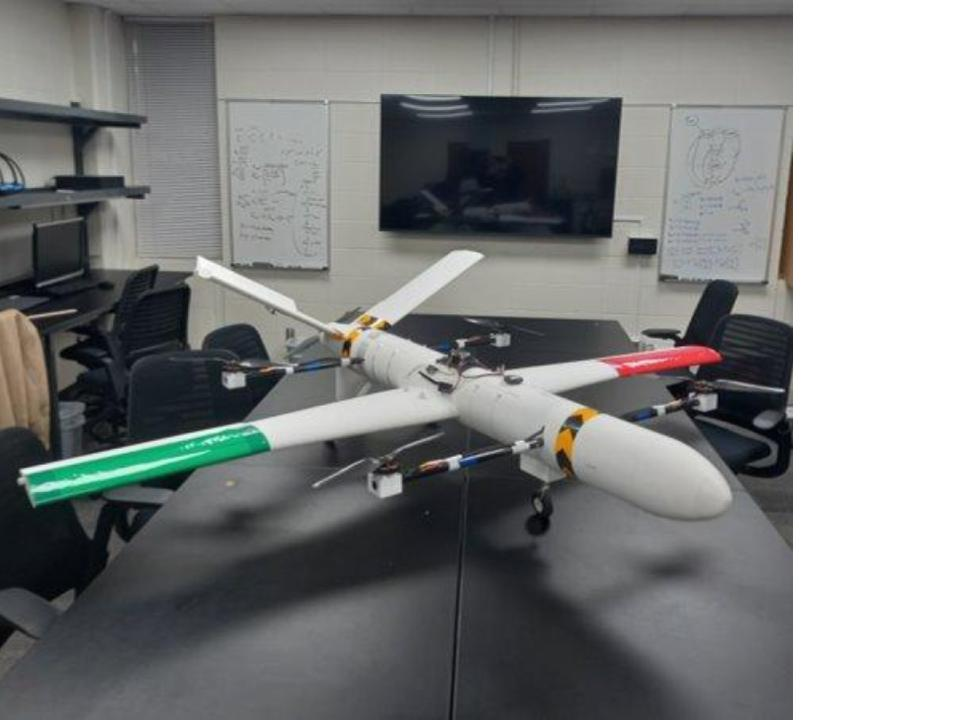
\includegraphics[width=\linewidth]{figs/chap1/quadplane.jpg}
    \caption{3D printed quadplane prototype for future use in autopilot tests.}
    \label{fig:quadplane3DPrinted}
\end{figure}

It is worthwhile developing controllers for the quadplane platform due to its relative simplicity, as it combines the two well-studied aircraft models of a fixed-wing airplane and a quadcopter. 
The aircraft can revert to a standard autopilot configuration, either quadrotor or airplane, as a failsafe in the case of failure of the experimental autopilot.

However, the quadplane is rather inefficient with its motor use.
The vertical motors are only used during for a short period during takeoff and landing, while the forward rotor does most of the long-range work.
Four of five motors are not used for the majority of the flight, which means a reduced payload due to the extra weight, and increased drag from the vertical rotors.
Some quadplanes use tilting mechanisms to utilize rotors as both vertical and forward thrusters, as described in \cite{tiltQuadplane}, though this adds complexity with the need for reliable motor tilting mechanisms.

Another promising VTOL is the tilt body design, as described in \cite{lou_unified_energy_control_tilt_body}. 
This aircraft has offset front and rear wings, with sets of propellers on both, as shown in Fig. \ref{fig:tiltbodyDesign}. 

\begin{figure}
    \centering
    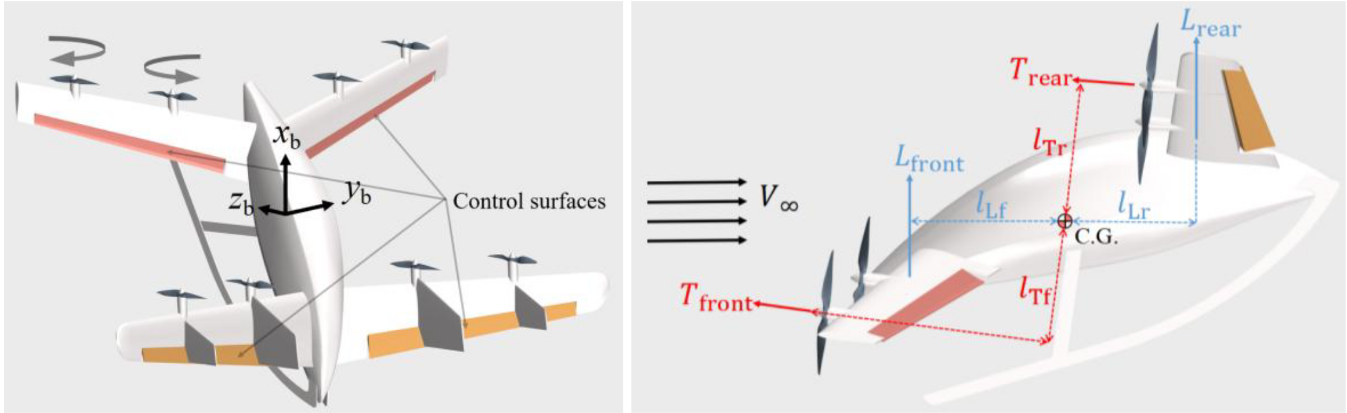
\includegraphics[width=\linewidth]{figs/chap1/tiltbodyDesign.png}
    \caption{Tiltbody design and configuration. Reproduced from \cite{lou_unified_energy_control_tilt_body} Fig. 3.}
    \label{fig:tiltbodyDesign}
\end{figure}

During takeoff, the two sets of rotors actuate differentially to rotate the aircraft to a vertical orientation for takeoff.
Using differential actuation of the rotors, the aircraft then rotates forward to move into fixed-wing flight. 
A diagram of these maneuvers is shown in \ref{fig:tiltbodyControl}.

\begin{figure}
    \centering
    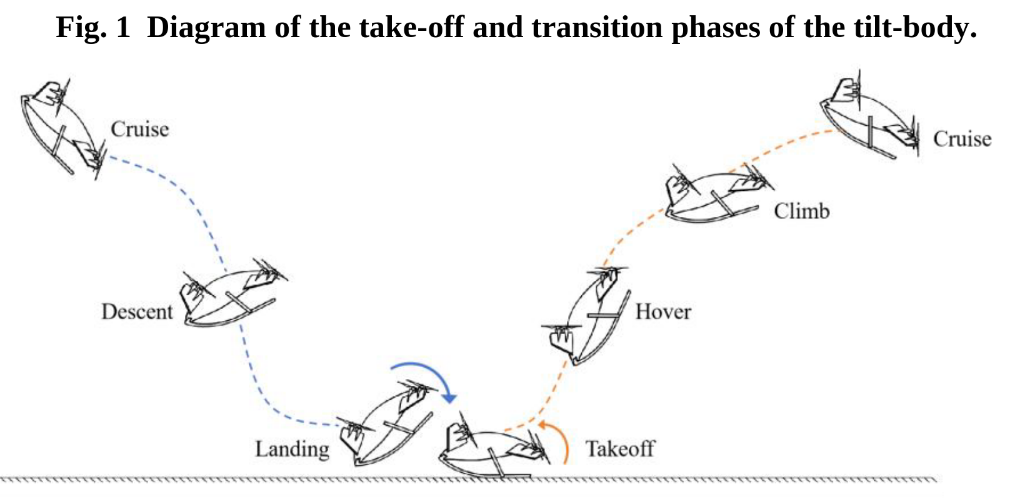
\includegraphics[width=\linewidth]{figs/chap1/tiltbodyManeuver.png}
    \caption{Tiltbody control map. Reproduced from \cite{lou_unified_energy_control_tilt_body} Fig. 2.}
    \label{fig:tiltbodyControl}
\end{figure}

This configuration of VTOL makes a more efficient use of all propellers, without the need for a motor rotating mechanism.
As tilt-body designs are not widely available for purchase, a 3D printed reproduction of this is currently being developed for future use and autopilot development in this research group.
The current design is shown in Fig. \ref{fig:tiltbodyAdamDesign}.

\begin{figure}
    \centering
    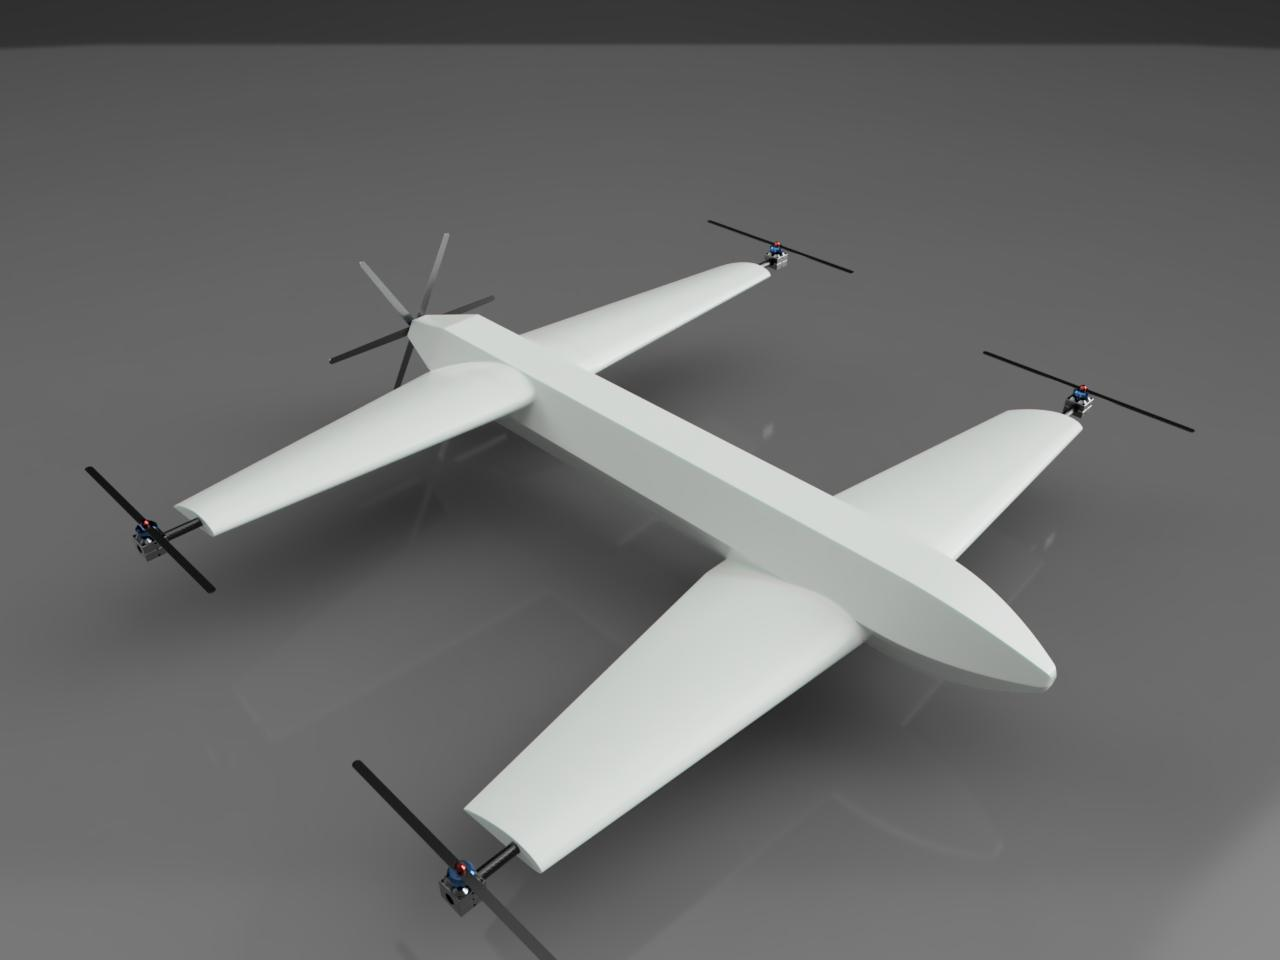
\includegraphics[width=\linewidth]{figs/chap1/Tandem Wing Design (Initial Render).jpg}
    \caption{Tiltbody CAD model for future 3D printing use.}
    \label{fig:tiltbodyAdamDesign}
\end{figure}

\subsection{Thrust Model}

It was assumed that the relationship between $\delta$ control input and thrust from the motor can be modeled as $T(\delta_t) = T_{max} \delta_t$. 
This was done for simplicity and stability in simulation. 
Section 4.3 on page 55 of Small Unmanned Aircraft \cite{uav_book} contains a more accurate aerodynamic thrust and moment model. 
Solutions for $\delta_t$ from these sets of equations would require another optimization step, which adds a potential failure point.
Hardware implementation will require implementation of this or another accurate thrust model.

\subsection{Computation}

At present, this controller stack is not ready for real-time hardware implementation due to the intensive computational burden. 
For example, when testing the autopilot for the takeoff controller, the following averages were obtained for each component of the controller.
The pitch-free trajectory tracker took $13.3 \space \mu s$, the pitch optimizer took $11.78 \space m s$, the moment controller took $15.9 \space \mu s$, and the elevator and thrust controllers took $145.0 \space \mu s$. 
This means an average time of $11.95 \space \mu s$ per update. 
For an autopilot operating at $100 Hz$, this is unreasonable, because computation alone is greater than the spacing between samples.
The most time-expensive component is pitch optization, which is apparent for this non-convex optimization.
Future implementations will require an autopilot with a significantly reduced computational burden for pitch optimization.

\section{Conclusion}

Study for control of VTOL aircraft will continue to increase in importance over the coming years. 
VTOL aircraft can fly long distances, due to their ability to operate like a fixed-wing aircraft. 
They do not require a runway for landing, but can take off and land vertically in quadcopter mode. 
Due to this flexibility, much research must be done to develop efficient controllers for transition from vertical to forward flight. 
Historically, the standard approach to this problem has been to fly to a high altitude in multi-copter mode, and then slowly increase forward throttle until the aircraft can generate enough lift to stay airborne. 

The new method presented in this paper is for a 2 Dimensional simplification of a standard quadplane. 
This simplification reduces the state of the aircraft from north ($n$), east ($e$), and down ($d$) to just $n$ and $d$. 
This reduces the rotations from roll ($\phi$), pitch ($\theta$), and yaw ($\psi$) about the $n$, $e$, and $d$ axes respectively to just pitch ($\theta$) about the fixed $e$ axis. 
This simplification was done due to the complex dynamics of the 3D eVTOL aircraft. 
Reducing the number of state variables enabled the research to be focused on the transition from vertical to forward flight. 

In this 2D simplification, a differentially flat autopilot was developed, with a positional trajectory reference.
This autopilot is divided into five segments: pitch-free trajectory tracking, pitch optimization, moment control, elevator allocation, and rotor allocation.
A positional trajectory is input to the system, which means that the position for each time step is referenced to the controller.
The reference velocity and acceleration may be calculated by taking derivatives of the reference position.

Pitch free trajectory tracking is a feedforward controller that calculates the desired force needed to keep the aircraft in the air following the trajectory.
It accomplishes this by directly matching the reference input acceleration and adding a constant gravity term, for the zero error case.
To overcome position and velocity error, a state error negative feedback control matrix $K$ is created using LQR to alter reference force.
This controller outputs a total reference force that must be achieved by the aircraft aircrame and rotors in the inertial frame, $F_{des}^i$. 

Pitch optimization minimizes the difference between total desired force and force achievable by the airframe airspeed and pitch by adjusting pitch $\theta$.
That is, it finds a reference pitch that maximizes aerodynamic lift.
This minimizes the lift that must be generated by the vertical rotors, which will minimize energy expenditure as the vertical quad rotors are less efficient than aerodynamic lift.
The optimization is performed using the 1-Norm in the objective function, which ensures a relatively quick transition from vertical to forward flight, and vice versa.
The output of this optimization are a reference pitch $\theta$ and a reference force for the aircraft rotors $f^b_{des,p}$.

The moment controller takes in reference pitch $\theta$ and outputs a reference pitch for the elevator and propellers to generate.
Moment control takes in the reference pitch from the previous section and finds its first and second derivatives, which are angular rate $q$ and angular acceleration $\dot{q}$.
This is another feedforward controller that sets the reference moment $M$ as the reference input angular acceleration $\dot{q}$ times the rotational inertia of the craft.
With the presence of pitch error $\tilde{\theta}$ and pitch rate error $\tilde{q}$, these will be compensated for using proportional and derivative terms $k_p$ and $k_d$.

From the output $M$ reference, the elevator controller attempts to find the input that will maximize moment generated by the elevator.
The elevator controller finds the difference between reference pitch and current feasible pitch and saturates to achieve the best moment.
The output from this controller is $\delta_e$, and the residual moment needed to be achieved by propeller differential $M_p$.

Finally the propeller control allocation takes in $f^b_{des,p}$ and $M_p$ to find the needed thrust and control inputs from the three rotors.
The thrust from the forward rotor is set to $f^b_{des,p,n}$.
The two vertical rotors use the inverted mixing matrix fo satisfy both $f^b_{des,p,d}$ and $M_p$.
The control inputs $\delta_f$, $\delta_r$, and $\delta_t$ are then calculated from the desired thrust by dividing by maximum thrust.

This controller was tested on several different flight paths. 
The first was a reference square root trajectory, which was tracked reasonably well and experienced a transition into forward flight.
The second was a reverse for a landing trajectory, which was unable to be tracked due to the saturation constraints of the forward thruster.
Others included the step error input, multiple inclines, and takeoff followed by a straight-line flight.

Each of these tests demonstrated the strengths and weaknesses of this aircraft setup.
Much more work must happen before this autopilot is ready to fly an actual VTOL.
